\chapter{Синтез моделей автоматных программ на основе сведения к задаче булевой выполнимости (SAT)}
\label{ch:automata-synthesis}

Данная глава посвящена решению задачи синтеза монолитных конечно-автоматных моделей логических контроллеров по примерам поведения и формальной спецификации.
В~разделе~\ref{sec:monolith-synthesis} предлагается метод синтеза по примерам поведения, основанный на сведении к задаче выполнимости SAT, приводится описание разработанных алгоритмов: $\AlgoBasic$ \--- для синтеза базовых моделей, $\AlgoExtended$ \--- для синтеза расширенных моделей, $\AlgoComplete$ \--- для учета негативных сценариев выполнения.
В~разделе~\ref{sec:monolith-minimal} рассматривается задача синтеза минимальных моделей, приводится описание разработанных алгоритмов $\AlgoBasicMin$, $\AlgoExtendedMin$, $\AlgoCompleteMin$ и $\AlgoExtendedMinUB$.
В~разделе~\ref{sec:monolith-cegis} рассматривается подход индуктивного синтеза, основанного на контрпримерах (\textit{Counterexample\-/Guided Inductive Synthesis} \--- CEGIS)~\cite{solar-lezama2006,abate2018}, используемый для учета при синтезе формальной спецификации, приводится описание алгоритмов $\AlgoCegis$ и $\AlgoCegisMin$.
Раздел~\ref{sec:experiments-monolith-pnp} содержит экспериментальное сравнение разработанных методов с существующими на примере задачи синтеза конечно-автоматной модели логического контроллера, управляющего Pick-and-Place манипулятором.
Раздел~\ref{sec:experiments-monolith-syntcomp} посвящен применению разработанных методов для минимизации \emph{систем переходов}, полученных с помощью программного средства для LTL-синтеза BoSy~\cite{bosy,not-bosy} по исходным данным с соревнования по реактивному синтезу SYNTCOMP~\cite{syntcomp}.
Все разработанные в данной работе методы реализованы в виде программного средства \smallcaps{fbSAT}~\cite{fbSAT-tool}.


\section{Фреймворк \texttt{kotlin-satlib}}

Для записи и передачи вышеописанного сведения в SAT-решатель в ходе выполнения данной работы была разработана специализированная программная библиотека \texttt{kotlin-satlib}\footnote{\url{https://github.com/Lipen/kotlin-satlib}}.
Разработанная библиотека выполнена в виде библиотеки на языке Kotlin и состоит из нескольких модулей: модуль взаимодействия с SAT-решателями через их нативные интерфейсы с помощью технологии JNI (\textit{Java Native Interface}), модуль для упрощенной записи распространенных видов ограничений с использованием преобразований Цейтина~\cite{tseitin1970}, модуль для манипуляции переменными с ограниченными доменами (например, целочисленными), а также модуль для манипуляции многомерными массивами SAT-переменных.
В~последующих разделах приведено описание этих модулей.

\subsection{Модуль взаимодействия с SAT-решателями на основе технологии JNI}

Практически все современные SAT-решатели предоставляют нативный программный интерфейс для взаимодействия с ними, однако так как подавляющее большинство решателей написаны на языках C/C++ (ввиду строгих требований к эффективности реализации), их прямое использование в языках более высокого уровня весьма затруднено.
В~данной работе в качестве целевой платформы используется JVM (\textit{Java Virtual Machine}), а именно, языки программирования Java и Kotlin.
Подавляющее большинство взаимодействий с нативным программным обеспечением из JVM так или иначе выполняется с помощью технологии JNI\footnote{\href{https://docs.oracle.com/javase/8/docs/technotes/guides/jni/}{https://docs.oracle.com/javase/8/docs/technotes/guides/jni}} (\textit{Java Native Interface}).
Данная технология позволяет описывать нативные методы (в~Java \--- с помощью ключевого слова \texttt{native}, в~Kotlin \--- с помощью ключевого слова \texttt{external}) в Java/Kotlin классах, реализация которых выполняется на нативном языке (обычно на C/C++), где уже можно получить доступ к другому нативному коду, например, к SAT-решаелям.
Полученные нативные реализации компилируются в динамические библиотеки (на GNU/Linux \--- \textit{shared object library}, на Windows \--- \textit{dynamic-link library}) и становятся доступными для виртуальной машины (JVM) во времени исполнения программы.

Сразу стоит отметить существование библиотеки jnisat на языке Java \--- программной обертки для решателей PicoSAT~\cite{biere2008} и MiniSAT~\cite{minisat}, использующей описанную технологию JNI.
Именно эта библиотека легла в основу фреймворка \texttt{kotlin-satlib}: собственная реализация была выполнена на языке Kotlin с поддержкой вызова кода из Java, был добавлен общий унифицированный интерфейс для SAT-решателей, а также была добавлена поддержка таких современных SAT-решателей, как MiniSat~\cite{minisat}, Glucose~\cite{glucose}, CryptoMiniSat~\cite{cryptominisat}, CaDiCaL~\cite{cadical} и Kissat~\cite{kissat}.

\subsection{Модуль записи ограничений с использованием преобразований Цейтина}

Практически все ограничения, определенные в разделе про кодирование задачи синтеза булевой формулы, не были представлены в конъюнктивной нормальной форме (КНФ), что затрудняет их прямую передачу в SAT-решатель \--- предварительно необходимо конвертировать все ограничения в набор дизъюнктов КНФ. Однако стоит учитывать, что некоторые выражения, например, вида $(x_{1} \land y_{1}) \lor \ldots \lor (x_{N} \lor y_{N})$, при конвертации их в эквивалентные КНФ имеют экспоненциальный размер (по числу дизъюнктов) относительно исходного.
Для решения этой проблемы можно воспользоваться неэквивалетными преобразованиями, которые сохраняют выполнимость формулы, так как при решении задачи SAT нас интересует только получаемая модель или же доказательство отсутствия решения.
Одними из наиболее известных таких преобразований являются преобразования Цейтина~\cite{tseitin1970}, основная идея которых \--- введение дополнительных переменных, кодирующих и заменяющих собой логические вентили в формуле, постепенно сводя ее к КНФ, размер которой растет полиномиально.
Например, для выражения $A \land B$ преобразование Цейтина вводит новую переменную $C \iff A \land B$, кодируемую в КНФ следующим образом:

\[(\neg A \lor \neg B \lor C) \land (A \lor \neg C) \land (B \lor \neg C)\]

Добавление новых переменных, безусловно, увеличивает теоретическую сложность задачи, однако на практике добавление дополнительных структурных ограничений может даже помочь ускорить процесс решения.
К тому же, современные SAT-решатели способны манипулировать миллионами переменных, поэтому применение преобразований Цейтина в случаях, когда наивная конвертация ограничений в КНФ приводила бы к экспоненциальному росту размера задачи, является целесообразным.

Разработанный фреймворк \texttt{kotlin-satlib} содержит модуль \texttt{Ops}, производящий такие преобразования Цейтина автоматически.
Модуль \texttt{Ops} также содержит множество типичных видов ограничений, например, функция \texttt{implyIffOr(x1:~Lit, x2:~Lit, xs:~Iterable<Lit>)} позволяет задать ограничение вида $x_{1} \implies (x_{2} \iff \biglorclap{x_{i} \in xs} x_{i}$).
Дополнительные перегрузки этих функций с альтернативными контейнерами используемых литералов, например, \texttt{implyIffOr(x1:~Lit, x2:~Lit, vararg xs:~Lit)}, образуют небольшой предметно-ориентированный язык (\textit{Domain Specific Language} \--- DSL), позволяющий пользователю сконцентрироваться на моделировании задачи и использовать практически произвольные виды ограничений, а не на механических действиях, связанных с кодированием дополнительных переменных и конвертацией ограничений в КНФ, необходимую для SAT-решателя.

\subsection{Модуль манипуляции переменными с ограниченным доменом}

Большинство переменных, определенных в разделе про кодирование задачи синтеза булевой формулы, не были логическими, а имели либо целочисленное значение из некоторого известного диапазона, либо некоторое значение из заданного множества допустимых, например, $\tau_{p} \in \{ \land, \lor, \neg, \bot \}$.
Стоит сразу отметить, что SAT-решатели поддерживают только логические переменные, однако на практике моделирование исходной задачи с использованием переменных с ограниченными доменами, а не только логических, зачастую оказывается гораздо более выразительным и позволяет смотреть на задачу с интуитивной стороны.
Основной подход к непосредственному кодированию переменных с ограниченным доменом \--- так называемое onehot-кодирование, при котором каждому возможному значению переменной из домена сопоставляется логическая переменная.
Например, истинная логическая переменная~$\tau_{p, \land}$ соответствует ситуации, когда $\tau_{p} = \land$.
При этом необходимо также добавить ограничение на то, что ровно один из \textit{onehot}-литералов может иметь истинное значение \--- это может быть сделано в виде комбинации ограничений AtLeastOne (не менее одного) и AtMostOne (не более одного).
Ограничение AtLeastOne является тривиальным и представляет из себя один дизъюнкт, содержащий все объявляенные литералы. А вот ограничение AtMostOne может быть закодировано множеством способов \--- от простых и интуитивных~\cite{walsh2000} до комплексных и эффективных~\cite{nguyen2015}, чему посвящены многочисленные исследования.

Стоит отметить, что \textit{onehot}-кодирование \--- далеко не единственный способ представления переменных в виде набора литералов, хотя и самый интуитивный и удобный в большинстве ситуаций. Среди альтернативных способов кодирования можно выделить следующие~\cite{sat-encodings}: порядковое (\textit{order encoding})~\cite{order-encoding}, бинарное (\textit{binary encoding}), комбинированное (\textit{onehot+binary encoding})~\cite{sat-encodings}.
Все такие способы обеспечивают некоторое представление исходной переменной с ограниченным доменом в SAT-решателе в виде набора литералов, однако различаются возможностями их использования в различных контекстах: \textit{onehot}-кодирование используется, когда необходимо получить доступ к значению переменной (здесь под \enquote{доступом} подразумевается использование переменной в декларативном процессе построения сведения); order-кодирование используется, если необходимо закодировать порядок между, например, целочисленными переменными; \textit{binary}-кодирование позволяет эффективно кодировать арифметические операции в сведении; гибридное \textit{onehot+binary}-кодирование обеспечивает комбинацию возможностей этих двух способов кодирования.

Описанные выше детали кодирования переменных с ограниченными доменами должны быть учтены при построении сведения, поэтому возникает желание автоматизировать эти действия.
Разработанный фреймворк \texttt{kotlin-satlib} содержит отдельный модуль \texttt{Vars}, предназначенный для манипуляции такими переменными.
Основой модуля является класс \texttt{DomainVar<T>}, хранящий набор литералов, соответствующих onehot-кодировке переменной со значениями произвольного типа \texttt{T}.
При создании экземпляра такой переменной имеется возможность указать один из способов кодирования: \textit{onehot} или \textit{onehot+binary}.
Класс \texttt{DomainVar<T>} также содержит инфиксные методы \texttt{eq(value:~T)} и \texttt{neq(value:~T)}, позволяющие обращаться к литералу, соответствующему значению \texttt{value}.
Например, пусть \texttt{v:~DomainVar<Int>}, тогда простое и удобное в использовании выражение `\texttt{v~eq~5}' соответствует литералу, кодирующему $v = 5$.

\subsection{Модуль манипуляции массивами SAT переменных}

Некоторые переменные сведения могут быть объявлены с множественными индексами, что подразумевает их хранение в многомерном массиве. Ввиду того, чт стандартные многомерные массивы, доступные в Java (например, \texttt{int[][][]}) и Kotlin (например, \texttt{Array<Array<Array<Int>>>}) не обеспечивают необходимой гибкости и удобств, была разработана собственная эффективная реализация многомерных массивов, оформленная в виде отдельной библиотеки MultiArray\footnote{\url{https://github.com/Lipen/MultiArray}} на языке Kotlin.

Библиотека MultiArray включает в себя набор интерфейсов и их реализаций для многомерных массивов, индексируемых с нуля или единицы (по выбору), хранящих либо значения произвольного типа, либо (в отдельных эффективных специализациях) целочисленные и булевы значения.
Основные интерфейсы, предоставляемые библиотекой \--- изменяемые (\texttt{Mutable\-Multi\-Array<T>}) и неизменяемые (\texttt{Multi\-Array<out~T>}) многомерные массивы.
Неизменяемая версия ковариантна по типу~\texttt{T}, что позволяет обращаться с такими массивами более гибко.
Внутри многомерных массивов данные хранятся в одном линейном массиве, а индексация происходит с помощью так называемых \textit{strides of array} (\enquote{шаги массива}).
Такой подход позволяет получить максимальную эффективность в совокупности с удобством по сравнению со стандартными массивами, встроенными в языки Java и Kotlin.


\section{Синтез булевых формул}
\label{sub:formula-synthesis}

Задача синтеза булевой формулы заключается в построении логической формулы, зависящей от $N$ переменных $x_{1}\ldots x_{N}$ (возможно, не от всех, то есть некоторые переменные могут не использоваться в полученной формуле), по заданной таблице истинности, с использованием заданных логических операций.
Заданная таблица истинности может быть как полной (размера~$2^{N}$), так и частичной \--- для некоторых наборов переменных (в~дальнейшем также называемых \enquote{входами}) значение логической функции может быть не определено.
Соответствующая логическая функция имеет ровно один логических выход, значения для которого на различных входах и записаны в таблице истинности.
Стоит отметить, что список допустимых логических операций может варьироваться, также как и возможность применения операций к подвыражениям, в зависимости от желаемого результата (например, формулы в так называемой нормальной форме отрицания (\textit{negation normal form}) могут содержать логическое отрицание, применяемое только к переменным, но не к комплексным выражениям).
В~данной работе рассматривается задача синтеза булевой формулы, содержащей следующие логические операции, без дополнительных ограничений на их применимость к подвыражениям: $\land$~(логическое~И), $\lor$~(логическое~ИЛИ) и $\neg$~(логическое отрицание).

В данной работе рассматривается задача синтеза минимальной булевой формулы, то есть формулы минимального размера, удовлетворяющей заданной таблице истинности.
Несмотря на простоту формулировки, задача синтеза минимальной булевой формулы по полной или частичной таблице истинности является NP-трудной~\cite{akshay2018}.
На практике данная задача обычно решается с помощью эвристических подходов, не гарантирующих минимального ответа.
Наиболее часто используемым подходом является использование метода Espresso~\cite{brayton1984}, реализация которого доступна в виде одноименного программного средства.
Несмотря на то, что этот эвристический подход был разработан относительно давно, его успех до сих пор не был существенно преодолен \--- многие современные подходы в той или иной степени являются модификациями Espresso, например, BOOM-II~\cite{fiser2006}.
Метод Espresso позволяет синтезировать \emph{минимальные} булевы формулы по заданным полным или частичным таблицам истинности, включая возможность синтезировать функции с множественными выходами.
В~процессе минимизации могут использоваться различные оптимизационные критерии, например, суммарное число логических вентилей или число использованных литералов.
Отличительной особенностью данного метода является его высокая эффективность.
Однако стоит отметить, что получаемое с помощью Espresso решение не является \emph{точным}, то есть не является наименьшим \--- возможно существование меньшего решения, даже при использовании большого числа итераций.
В~тех случаях, когда требуется \emph{точное} решение, то есть наименьшая из возможных булевых формул, необходимо использование других подходов, например, программирование в ограничениях, а именно, сведение к задаче выполнимости.

Для логической формулы может быть построено дерево разбора \--- укорененное (\textit{rooted}) дерево, во внутренних узлах которого находятся логические операции, а вершины-листья отмечены переменными $x_{1}\ldots x_{N}$.
Связи между вершинами соответствуют применению соответствующих операций к вершинам-потомкам.
Каждое поддерево такого дерева разбора может рассматриваться как некоторое подвыражение исходной формулы.
Размер дерева разбора \--- число вершин, из которых оно состоит (включая вершины-листья).
Размер логической формулы \--- размер соответствующего дерева разбора.
В дальнейшем размер дерева разбора или булевой формулы будет обозначаться как~$P$.

Сведение задачи к SAT обычно выглядит как декларативное описание с помощью логических переменных и ограничений структуры желаемого решения и его взаимодействия с исходными данными.
Вкратце, в случае рассматриваемой задачи синтеза булевой формулы от $N$~переменных, необходимо закодировать структуру дерева разбора синтезируемой формулы заданного размера~$P$, а также логические значения каждой вершины дерева разбора (каждая вершина соответствует некоторому подвыражению; корень дерева соответствует всей формуле) на различных входах.
После этого необходимо добавить ограничение на соответствие значений синтезируемой функции значениям в заданной таблице истинности.
Полученную в результате такого сведения SAT-формулу (в КНФ) необходимо решить с помощью SAT-решателя для получения либо искомой булевой формулы заданного размера~$P$, либо доказательства ее несуществования для заданного~$P$.

Для нахождения минимальной булевой формулы необходимо каким-либо образом определить минимальное значение~$P$, при котором решение существует.
Для этого в данной работе используется перебор параметра $P$ снизу вверх, начиная с единицы \--- таким образом, первое найденное решение будет минимальным из возможных.
При этом в данной работе используется два подхода: (1)~итеративный подход, при котором SAT-решатель перезапускается на каждом шаге для каждого нового значения~$P$; и (2)~инкрементальный подход, при котором на очередной итерации перебора параметра~$P$ сведение расширяется только теми ограничениями, которые зависят от нового значения~$P$, а вызовы SAT-решателя производятся с использованием предположений (\textit{assumptions}), что позволяет \emph{не перезапускать} SAT-решатель даже после получения UNSAT \--- сообщения об отсутствии решения при заданных ограничениях.

Рассмотрим подробнее составляющие сведения к SAT.
Параметр~$P$ отвечает за размер синтезируемой формулы \--- число вершин дерева разбора.
Вершины дерева разбора нумеруются последовательно, начиная с корневой, имеющей индекс~1.
В~общем случае порядок индексации вершин не имеет значения, однако на практике использование нумерации вершин дерева в порядке BFS-обхода (\textit{Breadth-First Search} \--- поиск в ширину) позволяет существенно сократить размер сведения, а также избавиться от большого числа изоморфных решений, что положительно влияет на эффективность метода \--- это так называемое \enquote{нарушение симметрий}~\cite{ulyantsev2015}, широко используемое при решении задач с помощью методов программирования в ограничениях.
Для обеспечения BFS-нумерации необходимо, во-первых, чтобы для любой пары смежных вершин дерева (родитель--потомок) номер родительской вершины был меньше номера потомка; а во-вторых, чтобы вершины-потомки нумеровались по порядку, без пропусков индексов.
В рассматриваемой задаче вершины могут иметь не более двух потомков \--- с номерами $c$ и $(c + 1)$, где~$c > p$.

Каждая вершина дерева может быть либо одной из допустимых логических операций ($\land, \lor, \neg$), либо терминалом, что кодируется с помощью переменной $\tau_{p} \in\nobreak \{\land, \lor, \neg, \bot\}$, где $p \in [1..P]$, а $\bot$~соответствует вершине-терминалу.
Переменная $\chi_{p} \in [0..N]$ кодирует номер переменной (от~1 до~$N$), которой соответствует вершина~$p$.
Только вершины-терминалы имеют ассоциированные переменные:
\[
    (\tau_{p} = \bot) \iff (\chi_{p} = 0)
\]

Переменная $\pi_{p} \in [0..(p - 1)]$, где $p \in [1..P]$, кодирует номер родительской вершины для вершины~$p$.
Как было упомянуто выше, номер родителя при использовании BFS-нумерации должен быть меньше номера самой вершины~$p$, поэтому доменом этой переменной является диапазон от 0 до $(p - 1)$.
При этом $\pi_{p} = 0$ означает, что у вершины~$p$ в дереве нет родителя \--- это выполняется только для корневой вершины.

Переменная $\sigma_{p} \in \{0\} \union [(p + 1)..P]$, где $p \in [1..P]$ кодирует номер левого потомка вершины~$p$.
Взаимосвязь между переменными $\pi$ и~$\sigma$ кодируется следующим образом:
\[
    (\sigma_{p} = c) \implies (\pi_{c} = p)
\]
В том случае, если тип вершины~$p$ \--- терминал, то такая вершина не имеет потомков:
\[
    (\tau_{p} = \bot) \implies (\sigma_{p} = 0)
\]
В~том случае, если вершина~$p$ имеет тип бинарной операции ($\land$~или~$\lor$), то вершина с номером $(\sigma_{p} + 1)$ неявно считается правым потомком вершины~$p$:
\[
    (\tau_{p} \in \{\land, \lor\}) \land (\sigma_{p} = c) \implies (\pi_{c + 1} = p)
\]

Переменная $\vartheta_{p,u} \in \Bool$ ($p \in [1..P]$, $u \in U$) кодирует логическое значение вершины~$p$ на входе~$u$.
Значение корневой вершины соответствует значению всей синтезируемой функции и должно совпадать со значением, указанным в заданной таблице истинности.
Значения вершин рассчитываются исходя из их типа, что декларативно можно описать следующими ограничениями:

\[
    (\tau_{p} = \bot) \land (\chi_{p} = x) \implies \biglandclap{u \in U} (\vartheta_{p,u} \iff u_{x})
\]

\[
    (\tau_{p} = \land) \land (\sigma_{p} = c) \implies \biglandclap{u \in U} (\vartheta_{p,u} \iff \vartheta_{c,u} \land \vartheta_{c + 1,u})
\]

\[
    (\tau_{p} = \lor) \land (\sigma_{p} = c) \implies \biglandclap{u \in U} (\vartheta_{p,u} \iff \vartheta_{c,u} \lor \vartheta_{c + 1,u})
\]

\[
    (\tau_{p} = \neg) \land (\sigma_{p} = c) \implies \biglandclap{u \in U} (\vartheta_{p,u} \iff {\neg\vartheta}_{c,u})
\]


\subsection{Экспериментальное исследование}

Был произведен синтез минимальных формул для всех 256 булевых функций от $X = 3$ переменных с использованием двух подходов поиска минимального значения параметра~$P$ \--- размера дерева разбора синтезируемой формулы: (1)~итеративный перебор с перезапуском SAT-решателя на каждом шаге (суммарное время \--- 171~с), (2)~инкрементальное расширение сведения с использованием предположений на каждом шаге (суммарное время \--- 185~с).
Результаты проведенного экспериментального сравнения представлены на Рисунке~\ref{fig:minbf} (слева), где оси соответствуют времени (в секундах, в логарифмической шкале) поиска минимальной булевой формулы двумя подходами, а каждая точка (всего 256 точек) соответствует отдельной булевой функции от $X = 3$ переменных.
Пунктирная красная линия (\textit{baseline}) соответствует равенству времени работы двух подходов.
Скопление точек сосредоточено около базовой линии, что свидетельствует о том, что оба подхода позволяют решать поставленную задачу примерно одинаково эффективно.

\begin{figure}[ht]
    \centering
    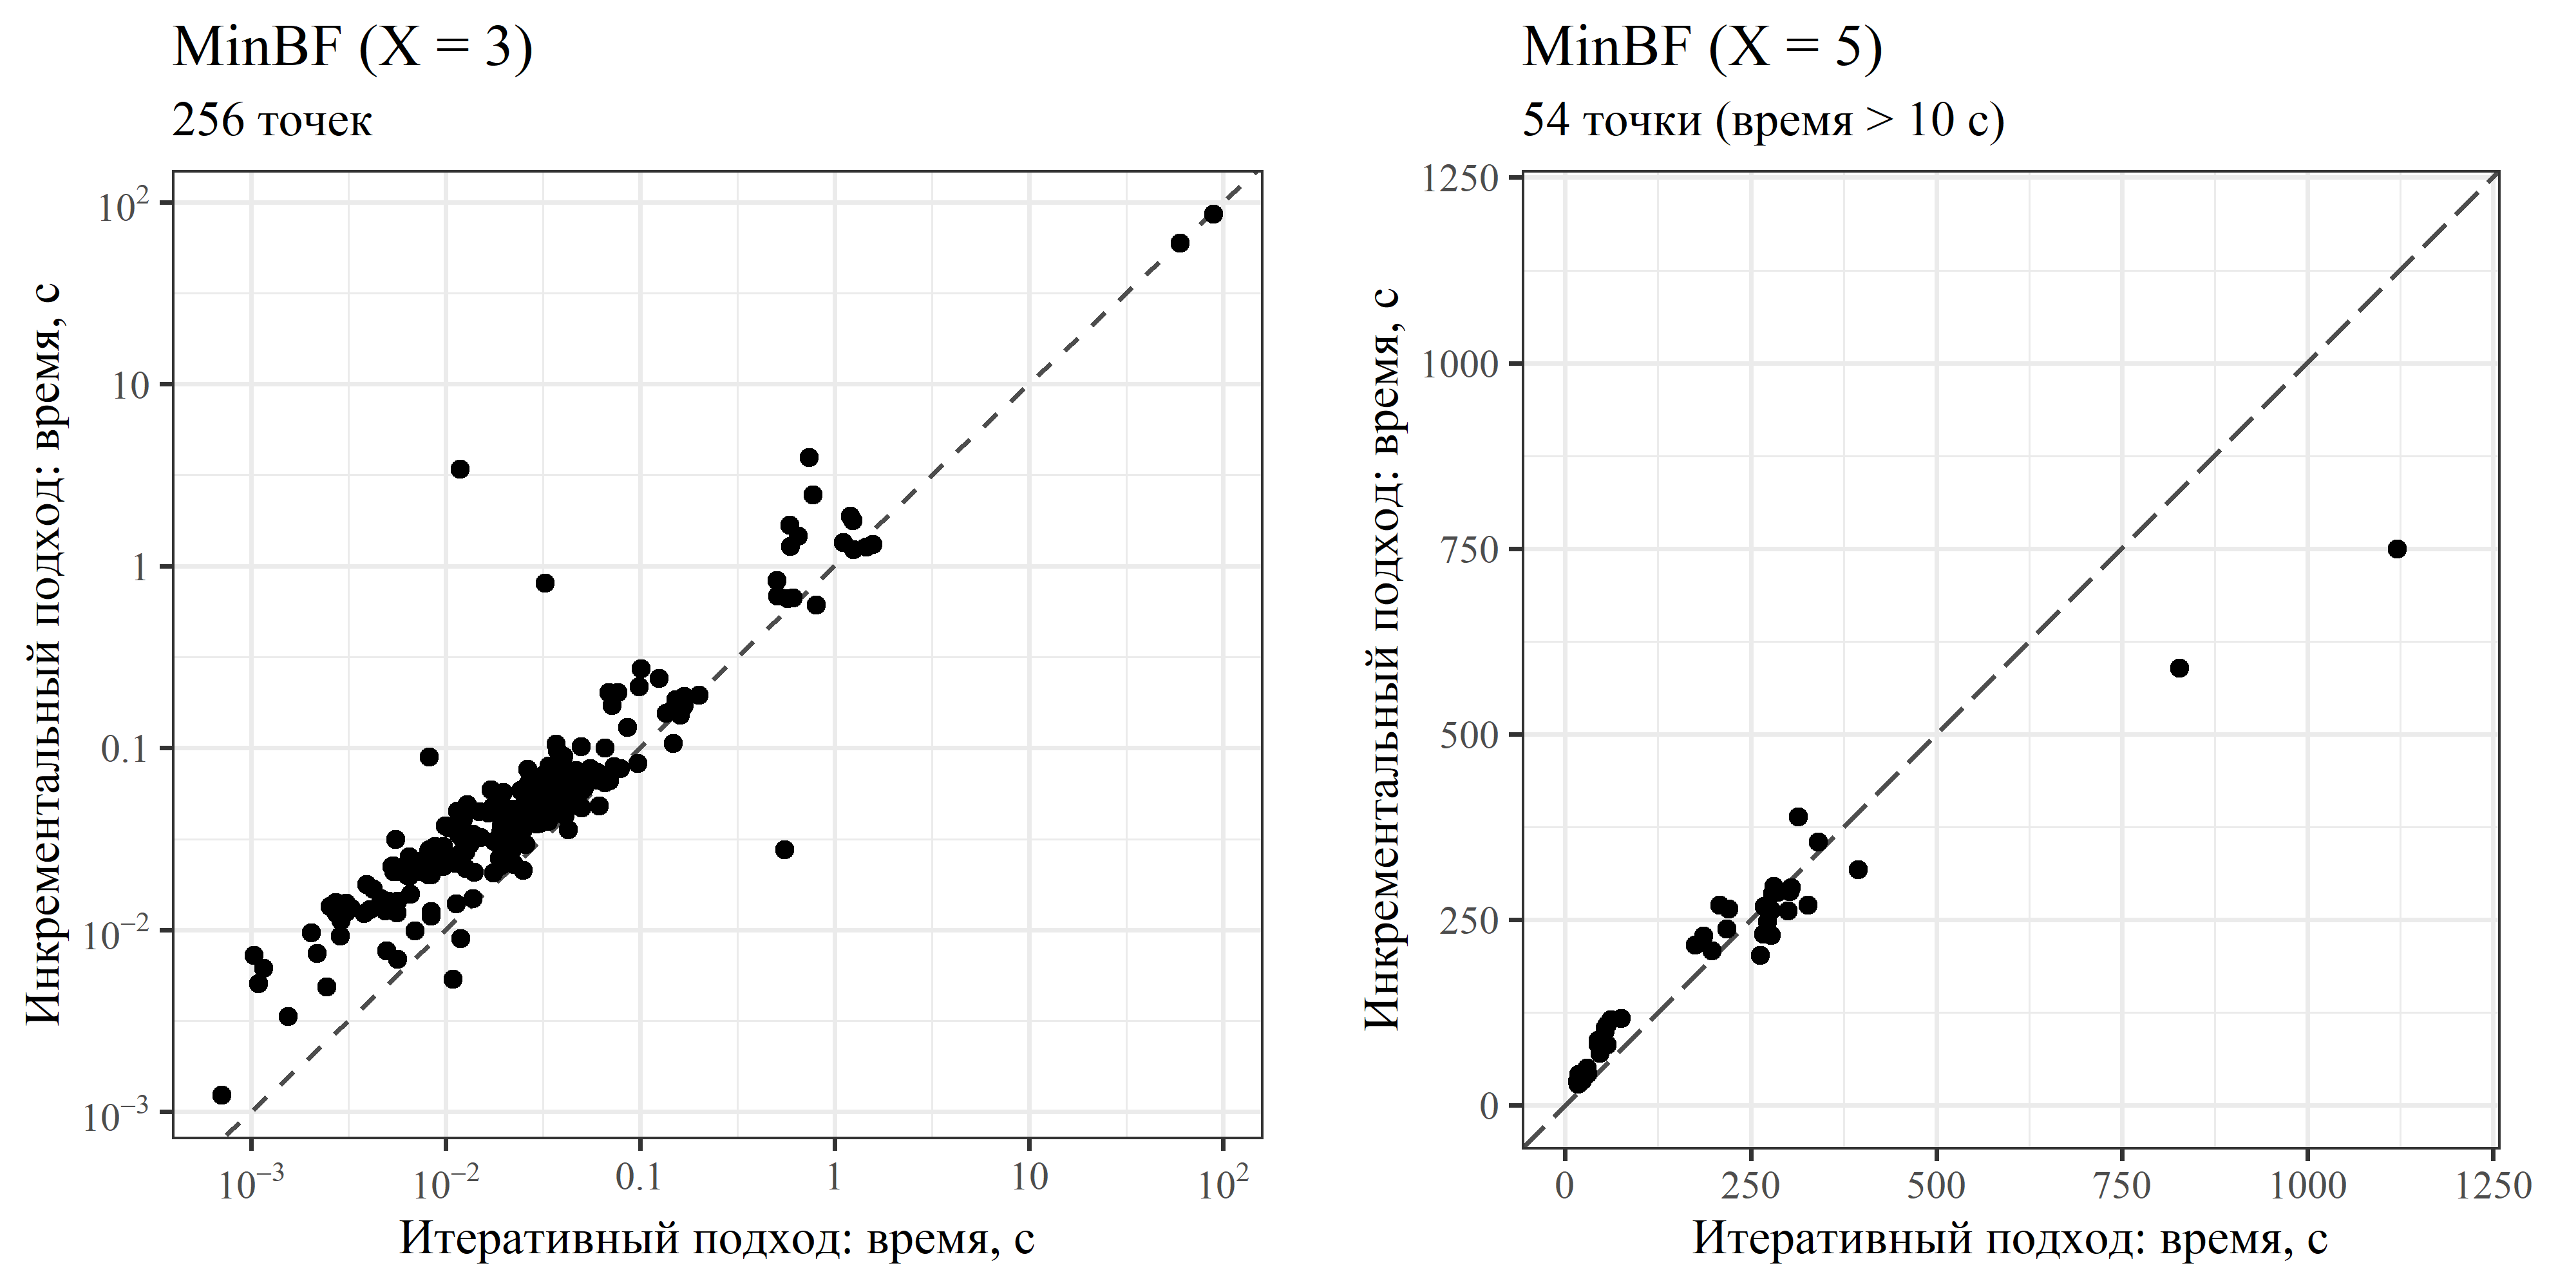
\includegraphics[max width=\linewidth]{minbf.png}
    \caption{Графики сравнения времени работы алгоритма синтеза минимальной булевой формулы (слева \--- от трех переменных, справа \--- от пяти переменных) для двух подходов: итеративный (горизонтальная ось) и инкрементальный (вертикальная ось). Время работы указано в секундах (слева \--- на логарифмической шкале). Каждая точка на графике соответствует булевой функции. На правом графике показаны только точки со временем работы, превышающим 10 секунд.}
    \label{fig:minbf}
\end{figure}

Можно заметить, что большинство минимальных формул для функций от трех переменных были найдены менее, чем за одну секунду \--- сравнение на таких масштабах времени в контексте решения NP-трудных задач не является целесообразным.
Поэтому были проведен дополнительный набор экспериментов на данных большей размерности и более \enquote{сложных} булевых функциях \--- от $X = 5$ переменных.
Результаты приведены на Рисунке~\ref{fig:minbf} (справа), где показаны только точки со временем работы, превышающим 10~секунд (всего 54~точки).
Данный график \--- а именно, точки в правой части графика под базовой линией \--- позволяет судить о том, что инкрементальный подход действительно обеспечивает лучшую производительность в рассмотренной задаче синтеза минимальной булевой формулы.


\section{Метод синтеза конечно-автоматных моделей монолитных логических контроллеров по примерам поведения}%
\label{sec:monolith-synthesis}

В этом разделе приводится описание разработанного метода синтеза минимальных моделей базовых функциональных блоков по примерам поведения и LTL\-/спецификации.
Сначала рассматривается решение базовой задачи (алгоритм $\AlgoBasic$) \--- синтеза моделей с использованием только сценариев выполнения \--- приводится описание переменных и ограничений, составляющих сведение к задаче SAT и предлагается итеративный подход к синтезу минимальных моделей.
Следом, сведение к SAT расширяется (алгоритм $\AlgoExtended$) кодированием структуры деревьев разбора произвольных булевых формул охранных условий, что приводит к возможности учета их суммарного размера при минимизации.
В заключение, решается задача синтеза модели, не только удовлетворяющей заданным примерам поведения, но и лишенной нежелательного поведения, выражаемого в виде негативных сценариев выполнения (алгоритм $\AlgoComplete$).
% После этого рассматривается подход индуктивного синтеза, основанного на контрпримерах (\textit{Counterexample\-/Guided Inductive Synthesis} \--- CEGIS), позволяющий решить (алгоритмы $\AlgoComplete$ и $\AlgoCegis$) поставленную задачу синтеза моделей одновременно по сценариям выполнения и LTL\-/спецификации.
% Разработанные методы реализованы в виде программного средства \smallcaps{fbSAT}~\cite{fbSAT-tool}.


\subsection{Кодирование структуры автомата}%
\label{sub:encoding-automaton-structure}

Сведение обозначенной задачи синтеза к задаче SAT заключается в построении булевой формулы, которая истина тогда и только тогда, когда существует конечный автомат размера $\card{\SetStates} = C$, удовлетворяющий заданному набору позитивных сценариев выполнения $\SetPositiveScenarios$.
Для этого необходимо рассмотреть процесс проверки соответствия автомата дереву сценариев и закодировать его в SAT\footnotemark.
\footnotetext{Здесь и далее фраза \enquote{закодировать в SAT} означает построение соответствующей булевой формулы в КНФ, кодирующей структуру и требуемые ограничения задачи синтеза.}
При этом также необходимо закодировать структуру синтезируемого объекта \--- конечного автомата, а точнее, ECC\@.
Здесь и далее в этом разделе предполагается, что $b \in \Bool = \Set{\top, \bot}$, $q \in \SetStates$, $k \in \Range{1}{K}$, $e \in \SetInputEvents$, $u \in \SetTreeInputs$, $v \in \SetTreeNodes$, если не указано иное.

Искомый автомат состоит из $C$ состояний, каждое из которых имеет ассоциированное \textit{действие} (выходное событие и алгоритм) и не более $K$ выходящих (\textit{outgoing}) переходов, упорядоченных в порядке их приоритета.
Выходное событие состояния $q \in \SetStates$ кодируется с помощью переменной $\StateOutputEvent{q} \in \SetOutputEvents \union \Set{\varepsilon}$.
% \footnote{Здесь и далее под кодирующей переменной подразумевается либо непосредственно булева переменная, либо набор булевых переменных, соответствующих значениям переменной с ограниченным доменом (например, при кодировании целочисленной переменной $x \in \Set{1,2,3}$ объявляются булевы переменные $x_1, x_2, x_3$}
Так как алгоритм является функцией, независимо изменяющей значения выходных переменных, то он кодируется с помощью переменной $\StateAlgorithm{q,z,b} \in \Bool$, где
$q \in \SetStates$ \--- состояние автомата,
$z \in \SetOutputVariables$ \--- выходная переменная,
$b \in \Bool$ \--- текущее значение выходной переменной.
Каждый переход в автомате ассоциирован с \textit{охранным условием} \--- парой из входного события и булевой формулы, зависящей от входных переменных $\SetInputVariables$ соответствующего базового функционального блока.
Переменная~$\TransitionDestination{q,k} \in \SetStatesAux = \SetStates \union \Set{q_0}$ кодирует конец $k$-го перехода из состояния~$q \in \SetStates$.
\enquote{Переходы} в фиктивное состояние~$q_0$ называются \textit{нулевыми} (\textit{null-transitions}) и означают отсутствие перехода в автомате.
Входное событие на переходе кодируется с помощью переменной $\TransitionInputEvent{q,k} \in \SetInputEvents \union \Set{\varepsilon}$.
Так как каждый переход должен обладать входным событием, то $\varepsilon$-событием отмечены только \textit{нулевые} (несуществующие) переходы: $(\TransitionDestination{q,k} = q_0) \iff (\TransitionInputEvent{q,k} = \varepsilon)$.
Переменная $\TransitionFiring{q,k,e,u} \in \Bool$ кодирует функцию активации охранного условия, то есть выполнение перехода при входном действии~$\Action{e}{u}$.
Переменная $\TransitionTruthTable{q,k,u} \in \Bool$ кодирует таблицу истинности охранного условия, то есть значение соответствующей булевой функции на входе $u \in \SetTreeInputs$.
Взаимосвязь между этими переменная задается следующим образом:
\[
    \TransitionFiring{q,k,e,u}
    \iff
    (\TransitionInputEvent{q,k} = e)
    \land
    \TransitionTruthTable{q,k,u} .
\]

В соответствии со стандартом IEC~61499, переходы ECC обладают приоритетом.
Переменная $\TransitionFirstFired{q,e,u} \in \Range{0}{K}$ кодирует индекс перехода, который выполняется \textit{первым} при входном действии $\Action{e}{u}$ \=== только этот переход будет учтен в момент исполнения ECC, даже если следующие переходы также выполняются.
При этом $\TransitionFirstFired{q,e,u} = 0$ означает, что \emph{ни один} переход не выполняется при входном действии~$\Action{e}{u}$.
Некоторый $k$-й переход выполняется \emph{первым} тогда и только тогда, когда (1)~он выполняется ($\TransitionFiring{q,k,e,u} = \top$) и (2)~не выполняются все предыдущие ($k' < k$) переходы.
Наивный способ кодирования переменной~$\TransitionFirstFired*$ выглядит следующим образом:
\[
    (\TransitionFirstFired{q,e,u} = k)
    \iff
    \TransitionFiring{q,k,e,u}
    \land
    \biglandclap{1 \leq k' < k}
    (\neg\TransitionFiring{q,k',e,u}) .
\]
Более эффективный способ кодирования заключается в определении специальной переменной~$\TransitionNotFired{q,k,e,u} \in \Bool$ для кодирования того факта, что все переходы с~1 по~$k$-й не выполняются.
При этом можно заметить, что такая переменная может быть определена рекурсивно:
\[
    \TransitionNotFired{q,k,e,u}
    \iff
    \neg\TransitionFiring{q,k,e,u}
    \land
    \TransitionNotFired{q,k-1,e,u} ,
\]
где следует считать, что $\TransitionNotFired{q,0,e,u} = \bot$.
Исходя из этого, эффективный способ кодирования переменной~$\TransitionFirstFired*$ выглядит следующим образом:
\[
    (\TransitionFirstFired{q,e,u} = k)
    \iff
    \TransitionFiring{q,k,e,u}
    \land
    \TransitionNotFired{q,k-1,e,u} .
\]


% TODO: ограничения

Рассмотрим сценарий выполнения $s \in \SetPositiveScenarios$ и автомат~$\Automaton$, изначально находящийся в стартовом состоянии~$\InitialState$.
Автомат последовательно обрабатывает входные действия из сценария и, возможно (если выполняется какой-либо переход, то есть соответствующее охранное условие становится истинным), изменяет состояние, продуцируя выходные действия.
Когда автомат находится в состоянии~$q$ и обрабатывает входное действие~$\InputAction$, он либо (1)~переходит в состояние~$q'$, либо (2)~\enquote{игнорирует} входное действие, оставаясь в том же состоянии.
Такое поведение описывается переменной $\ActualTransitionFunction{q,e,u} \in \SetStatesAux$, где $\ActualTransitionFunction{q,e,u} = q_0$ соответствует второму~(2) случаю.
Заметим, что в первом случае автомат может перейти по переходу-петле и остаться в исходном состоянии $q' = q$, что, однако, отличается от случая $q' = q_0$, при котором не происходит генерации выходного действия, ассоциированного с состоянием~$q$.


\subsection{BFS-предикаты нарушения симметрии для состояний автомата}%
\label{sub:encoding-bfs-automaton}

Дополнительно, стоит добавить ограничения нарушения симметрии (\textit{symmetry breaking predicates})~\cite{ulyantsev2015}, форсирующие нумерацию состояний автомата в порядке BFS-обхода (\textit{breadth-first search}), то есть в том порядке, в котором они были бы посещены при выполнении поиска в ширину из стартового состояния.
Такие ограничения позволяют существенно сократить пространство поиска, что позитивно влияет на время решения задачи SAT.
Стоит отметить, что данные ограничения не влияют на корректность решения \--- если решение существует, то оно будет найдено независимо от нумерации состояний автомата.

Суть BFS-предиката нарушения симметрии заключается в следующем наблюдении относительно дерева BFS-обхода: родителем каждой вершины может быть только вершина с меньшим номером, а потомки каждой вершины следуют в строгом возрастающем порядке \--- номера соседних (\textit{sibling}) вершин отличаются на~1.
Из~этого следует, что для каждой вершины $i > 1$ верно следующее: родитель соседней ($i + 1$) вершины либо совпадает с родителем вершины~$i$, либо имеет больший номер.
Для кодирования такого ограничения в SAT, необходимо объявить следующие переменные.
Переменная $\BfsTransitionAutomaton{q_i,q_j} \in \Bool$ ($q_i,q_j \in \SetStates$) кодирует наличие любого перехода из~$q_i$ в~$q_j$ в автомате:
\[
    \BfsTransitionAutomaton{q_i,q_j}
    \iff
    \biglorclap{k \in \Range{1}{K}}
    (\TransitionDestination{q_i,k} = q_j) .
\]
Переменная $\BfsParentAutomaton{q_j} \in \Set{q_1,\dotsc,q_{j-1}}$ ($q_j \in \SetStates$) кодирует родителя вершины~$q_j$ в дереве BFS-обхода:
\[
    (\BfsParentAutomaton{q_j} = q_i)
    \iff
    \BfsTransitionAutomaton{q_i,q_j}
    \land
    \biglandclap{r < i}
    \neg \BfsTransitionAutomaton{q_r,q_j} .
\]
Непосредственно BFS-ограничение выглядит следующим образом:
\[
    (\BfsParentAutomaton{q_j} = q_i)
    \implies
    (\BfsParentAutomaton{q_{j+1}} \geq q_i) .
\]

Можно заметить, что в BFS-ограничении присутствует отношение $(\BfsParentAutomaton{q_{j+1}} \geq q_i)$.
Наивный способ кодирования такого ограничения в SAT выглядит следующим образом:
\[
    (\BfsParentAutomaton{q_j} = q_i)
    \implies
    \biglandclap{r < i}
    (\BfsParentAutomaton{q_{j+1}} \neq q_r) .
\]
Однако существуют и другие, теоретически более эффективные способы.
Например, можно использовать так называемые \enquote{переменные, кодирующие порядок} (\textit{order-encoding})~\cite{order-encoding}.
Перед тем, как перейти к их описанию, необходимо напомнить, что привычные переменные с ограниченным доменом, например, $x \in \Set{2, 3, 5}$, кодируются следующим образом, называемым в разных источниках как \enquote{\textit{onehot}}, \enquote{\textit{sparse encoding}}, \enquote{\textit{direct encoding}}~\cite{direct-encoding}, \enquote{\textit{pairwise encoding}}: для каждого значения из домена создается отдельная булева переменная, кодирующая равенство переменной этому значению, например, $x \mathrel{\mathord{\bowtie}_{\mathit{onehot}}} \Set{x_2, x_3, x_5}$, где $x_2 \equiv (x = 2)$, $x_3 \equiv (x = 3)$, $x_5 \equiv (x = 5)$.
Аналогичным образом определяются и \textit{order-encoded} переменные, однако кодируют они не равенство, а отношение порядка, например, $x \mathrel{\mathord{\bowtie}_{\mathit{order}}} \Set{x'_2, x'_3, x'_4, x'_5}$, где $x'_i \equiv (x \geq i)$.
Заметим, что на практике домены переменных являются непрерывными\footnote{Под \enquote{непрерывным} доменом здесь подразумевается дискретная последовательность без \enquote{пропусков}, что в случае численных доменов выражается в виде интервала $\Range{\text{low}}{\text{high}}$.}, поэтому кодирующих переменных будет столько же, сколько и при \textit{onehot}-кодировании\footnote{Можно заметить, что в рассмотренном примере переменная $x'_2 \equiv (x \geq 2)$ всегда истинна, а значит ее можно не вводить, поэтому корректнее говорить, что \textit{order-encoded} переменных всегда на одну меньше \textit{onehot}.}.
Детальное описание \textit{order encoding} присутствует в~\cite{order-encoding} и в данной работе не приводится.
Таким образом, BFS-предикат с использованием \textit{order-encoded} переменной $\BfsParentAutomaton[\mathit{(order)}]{q_j} \equiv (\BfsParentAutomaton{q_j} \geq q_j)$ может быть сформулирован следующим образом:
\[
    (\BfsParentAutomaton{q_j} = q_i)
    \implies
    \BfsParentAutomaton[\mathit{(order)}]{q_i}
\]
К сожалению, данное усовершенствование не привело к видимым изменениям производительности сведения (результаты экспериментального исследования не приводятся), поэтому здесь и далее в данной работе считается, что используется наивный способ кодирования BFS-предиката нарушения симметрии.


\subsection{Кодирование отображения позитивного дерева сценариев}%
\label{sub:encoding-positive-mapping}

%% Picture: Tree-to-automaton mapping
\begin{figure}
    \centering
    \begin{adjustbox}{max width=\linewidth}
        \subfile{tex/tikz-mapping}%
    \end{adjustbox}
    \caption{Пример отображения дерева сценариев на автомат}%
    \label{fig:tree-automaton-mapping}
\end{figure}

Для обеспечения соответствия автомата дереву сценариев, необходимо построить отображение $\Mapping* \colon \SetTreeNodes \to \SetStates$ вершин дерева на состояния автомата.
Пример такого отображения приведен на рисунке~\ref{fig:tree-automaton-mapping}.
Переменная $\Mapping{v} \in \SetStates$ кодирует \textit{удовлетворяющее состояние}, в котором автомат оказывается после обработки вершины дерева $v \in \SetTreeNodes$.
Корень дерева $\TreeRoot$ отображается в стартовое состояние автомата: $\Mapping{\TreeRoot} = \InitialState$.
Пассивные вершины ($\toe{v} = \varepsilon$) соответствуют ситуации, когда автомат должен проигнорировать входное действие, не изменяя своего состояния, что может быть выражено с помощью следующих ограничений: $\Mapping{v} = \Mapping{p}$ и $\ActualTransitionFunction{q,e,u} = q_0$, где $v \in \SetTreeNodesPassive$, $p = \tp{v}$, $q = \Mapping{p}$, $e = \tie{v}$, $u = \tin{v}$.
Активные вершины ($\toe{v} \neq \varepsilon$) соответствуют ситуации, когда автомат должен отреагировать на входное действие и продуцировать определенное (непустое) выходное действие, что может быть закодировано следующим образом:
\[
    (\Mapping{v} = q')
    \implies
    (\ActualTransitionFunction{q,e,u} = q')
    \land
    (\StateOutputEvent{q'} = o)
    \land
    \biglandclap{z \in Z}
    (\StateAlgorithm{q',z,b} = b') ,
\]
где $v \in \SetTreeNodesActive$, $p = \tp{v}$, $q = \Mapping{p}$, $q' \in \SetStates$, $e = \tie{v}$, $u = \tin{v}$, $o = \toe{v}$, $z \in Z$, $b = \tov{p,z}$, $b' = \tov{v,z}$.


\subsection{Кодирование ограничений на количество переходов}%
\label{sub:encoding-transitions-bounds}

Для того, чтобы ограничить количество переходов в автомате, то есть закодировать ограничение вида \enquote{суммарное число \emph{ненулевых} переходов в автомате не больше~$T$}, можно воспользоваться техникой \textit{totalizer} (раздел~\ref{sec:cardinality}) и закодировать в SAT \textit{ограничение на кардинальность}~$\Phi(\mathcal{D}, 0, T)$, где $\mathcal{D} = \Set{ \TransitionDestination{q,k} \neq q_0 \given q \in \SetStates, k \in \Range{1}{K} }$ \--- множество интересующих переменных, $T$ \=== верхняя граница для суммарного числа ненулевых переходов в автомате.
Стоит отметить, что на практике интерес представляет задача минимизации числа переходов в автомате, рассматриваемая в данной работе далее, поэтому нижняя граница принимается равной нулю.
Техника \textit{totalizer} позволяет кодировать сразу две границы, что может быть полезно при иных постановках задачи \--- например, возможно синтезировать автомат с точным (заранее известным) числом переходов~$T^{*}$, для чего необходимо закодировать обе границы, равные~$T^{*}$ \--- однако такие задачи в данной работе не рассматриваются.


\subsection{Алгоритм \AlgoBasic}%
\label{sub:algorithm-basic}

Описанные выше переменные и ограничения позволяют синтезировать \emph{вычислимые} конечно-автоматные модели, то есть модели, способные реагировать на входные воздействия, генерируя выходные действия.
Обозначим $\AlgoBasicFull(\SetPositiveScenarios, C, T)$ процедуру нахождения автомата, который удовлетворяет заданному набору позитивных сценариев выполнения~$\SetPositiveScenarios$, и в котором~$C$ состояний и суммарно не более~$T$ переходов.
Данная процедура состоит из (1)~построения позитивного дерева сценариев~$\PositiveTree$, (2)~формирования сведения к SAT (кодирование структуры автомата, отображения дерева сценариев и ограничения на кардинальность) и (3)~вызова SAT-решателя.
Результатом работы данной процедуры является либо искомый конечный автомат, либо доказательство отсутствия автомата заданного размера.
Также введем обозначение $\AlgoBasic(\SetPositiveScenarios, C) = \AlgoBasicFull(\SetPositiveScenarios, C, T=\infty)$ для случая, когда число переходов в автомате остается неограниченным.
Стоит отметить, что параметр~$K$ \--- максимальное число переходов из каждого состояния \--- здесь и далее принимается равным $K = C \cdot \card{\SetInputEvents}$, так как при меньших значениях возможно отсутствие решения из-за слишком сильных ограничений на искомую модель, а дополнительный перебор подходящего значения~$K$ является обременительной задачей.
% Также стоит отметить, что уменьшение параметра~$K$ значительно сокращает размер сведение, а значит, увеличивает эффективность решения задачи синтеза, поэтому любые оценки данного параметра могут быть исключительно полезны.


\subsection{Кодирование структуры охранных условий}%
\label{sub:encoding-guards-structure}

В вышеописанном сведении охранные условия представляются в виде таблиц истинности соответствующих булевых формул \--- посредством переменной~$\TransitionTruthTable*$.
Однако такие охранные условия сложны для восприятия человеком, а также неприменимы в средствах разработки систем управления, таких так Matlab или nxtSTUDIO~\cite{nxtstudio}, где охранные условия должны быть явно представлены в виде булевых формул.
Поэтому сведение расширяется кодированием деревьев разбора произвольных булевых формул, зависящих от входных переменных $\SetInputVariables$.

Каждое дерево разбора охранного условия на $k$-м переходе ($k \in\nobreak \Range{1}{K}$) из состояния $q \in \SetStates$ состоит из~$P$ вершин, где~$P$ является параметром разрабатываемого метода.
Каждая вершина типизирована и может быть либо булевым оператором, либо терминальной вершиной, соответствующей входной переменной.
Здесь стоит отметить, что параметр~$P$ является \enquote{глобальным} для всего автомата, то есть \emph{все} охранные условия состоят из~$P$ вершин.
Так как существуют булевы формулы, для записи которых достаточно менее~$P$ вершин в дереве разбора, некоторые вершины могут быть \enquote{нетипизированными} (\textit{none-typed}), то есть не включаться в дерево.
Размер дерева разбора определяется как число \emph{типизированных} вершин в нем.
Здесь и далее будут использованы следующие обозначения, если не указано иное: $p \in \Range{1}{P}$, $x \in \SetInputVariables$, $u \in \SetTreeInputs$.

Переменная $\NodeType{q,k,p} \in \Set{\NodeTypeTerminal, \NodeTypeAnd, \NodeTypeOr, \NodeTypeNot, \NodeTypeNone}$ кодирует тип вершины дерева разбора~$p$, где \enquote{$\NodeTypeTerminal$} обозначает терминальные вершины, \enquote{$\NodeTypeAnd$}, \enquote{$\NodeTypeOr$}, \enquote{$\NodeTypeNot$} \--- логические операторы, а \enquote{$\NodeTypeNone$} \--- нетипизированные вершины.
Без потери общности можно задать ограничение на то, что нетипизированные вершины имеют наибольшие номера в дереве: $(\NodeType{q,k,p} =\nobreak \NodeTypeNone) \implies (\NodeType{q,k,p+1} =\nobreak \NodeTypeNone)$.
Переменная $\NodeInputVariable{q,k,p} \in\nobreak \SetInputVariables \union\nobreak \Set{0}$ кодирует входную переменную (или ее отсутствие: $\NodeInputVariable{q,k,p} = 0$), ассоциированную с терминальной вершиной $p$.
Только терминальные вершины могут иметь ассоциированные входные переменные:
\[
    (\NodeType{q,k,p} = \NodeTypeTerminal) \iff (\NodeInputVariable{q,k,p} \neq 0)
\]

Для задания структуры дерева разбора, а именно, для определения родительских связей между вершинами, используются переменные $\NodeParent{q,k,p} \in\nobreak \Range{0}{(p-1)}$ и~$\NodeChild{q,k,p} \in\nobreak \Set{0} \union \Range{(p+1)}{P}$, кодирующие, соответственно, родителя и \emph{левого} ребенка вершины~$p$ (либо их отсутствие: $\NodeParent{q,k,p} = 0$, $\NodeChild{q,k,p} = 0$).
Взаимосвязь между этими переменными задается следующим образом:
\[
    (\NodeChild{q,k,p} = ch) \implies (\NodeParent{q,k,ch} = p)
\]
Только типизированные вершины, кроме корня ($p = 1$), имеют родительские вершины:
\[
    (\NodeParent{q,k,p} \neq 0) \iff (\NodeType{q,k,p} \neq \NodeTypeNone)
\]
Стоит отметить, что правый ребенок вершины дерева разбора не кодируется явно \--- для бинарных операторов предполагается, что он имеет номер на единицу больше левого ребенка ($c \in\nobreak \Range{(p+1)}{(P-1)}$):
\[
    (\NodeType{q,k,p} \in \Set{\NodeTypeAnd, \NodeTypeOr})
    \land
    (\NodeChild{q,k,p} = c)
    \implies
    (\NodeParent{q,k,c+1} = p) .
\]

Переменная $\NodeValue{q,k,p,u} \in \Bool$ кодирует значение подформулы \--- булевого выражения, соответствующего поддереву с корнем~$p$ \--- на входе~$u$.
Значение корня дерева разбора соответствует значению всей булевой формулы охранного условия, а значит, можно переиспользовать переменную~$\TransitionTruthTable{q,k,u}$, объявленную ранее: $\TransitionTruthTable{q,k,u} \equiv \NodeValue{q,k,1,u}$.
Значения терминальных вершин соответствуют значениям ассоциированных входных переменных;
значения вершин-операторов могут быть вычислены на основе значений вершин-потомков;
значения нетипизированных вершин для определенности принимаются равными \texttt{False}, однако это является лишь технической деталью реализации \--- значения нетипизированных вершин впоследствии не используются:
\begin{align*}
    (\NodeType{q,k,p} = \NodeTypeTerminal) \land (\NodeInputVariable{q,k,p} = x)
    &\implies
    \biglandnolim_{u \in \SetTreeInputs}
    \left[
        \NodeValue{q,k,p,u}
        \iff
        u_x
    \right] ;
\\
    (\NodeType{q,k,p} = \NodeTypeAnd) \land (\NodeChild{q,k,p} = c)
    &\implies
    \biglandnolim_{u \in \SetTreeInputs}
    \left[
        \NodeValue{q,k,p,u} \iff \NodeValue{q,k,c,u} \land \NodeValue{q,k,c+1,u}
    \right] ;
\\
    (\NodeType{q,k,p} = \NodeTypeOr) \land (\NodeChild{q,k,p} = c)
    &\implies
    \biglandnolim_{u \in \SetTreeInputs}
    \left[
        \NodeValue{q,k,p,u} \iff \NodeValue{q,k,c,u} \lor \NodeValue{q,k,c+1,u}
    \right] ;
\\
    (\NodeType{q,k,p} = \NodeTypeNot) \land (\NodeChild{q,k,p} = c)
    &\implies
    \biglandnolim_{u \in \SetTreeInputs}
    \left[
        \NodeValue{q,k,p,u} \iff \neg\NodeValue{q,k,c,u}
    \right] ;
\\
    (\NodeType{q,k,p} = \NodeTypeNone)
    &\implies
    \biglandnolim_{u \in \SetTreeInputs}
    \left[
        \neg\NodeValue{q,k,p,u}
    \right] .
\end{align*}


\subsection{BFS-предикаты нарушения симметрии для охранных условий}%
\label{sub:encoding-bfs-guards}

Дополнительно, стоит добавить ограничения нарушения симметрии, форсирующие BFS-нумерацию вершин дерева разбора охранного условия.
Фактически, они аналогичны BFS-ограничениям для состояний автомата (раздел~\ref{sub:encoding-bfs-automaton}), но применяются не ко всему автомату, а к каждому дереву разбора охранного условия по-отдельности: для каждого $q \in \SetStates$, $k \in \Range{1}{K}$.
Переменная $\BfsTransitionGuard{i,j} \in \Bool$ (${1 \leq i < j \leq P}$) задает существование \enquote{перехода} из $i$-й вершины в~$j$-ю:
\[
    \BfsTransitionGuard{i,j}
    \iff
    (\NodeParent{q,k,j} = i) .
\]
Переменная $\BfsParentGuard{j} \in \Range{1}{(j-1)}$ ($j \in \Range{2}{P}$) кодирует родителя $j$-й вершины в дереве BFS-обхода:
\[
    (\BfsParentGuard{j} = i)
    \iff
    \BfsTransitionGuard{i,j}
    \land
    \biglandclap{r < i}
    \neg \BfsTransitionGuard{r,j} .
\]
Непосредственно BFS-ограничение задается следующим образом:
\[
    (\BfsParentGuard{j} = i)
    \implies
    % just relation?
    \biglandclap{r < i}
    (\BfsParentGuard{j+1} \neq r) .
\]


\subsection{Кодирование ограничений на суммарный размер охранных условий}%
\label{sub:encoding-guards-bounds}

Для того, чтобы ограничить размер охранных условий в автомате, то есть закодировать ограничение вида \enquote{суммарное число \emph{типизированных} вершин в деревьях разбора булевых формул, соответствующих охранным условиям на переходах автомата не больше~$N$}, можно воспользоваться техникой \textit{totalizer} (см.~раздел~\ref{sec:cardinality}) и закодировать в SAT \textit{ограничение на кардинальность}~$\Phi(\mathcal{H}, 0, N)$, где $\mathcal{H} = \Set{ \NodeType{q,k,p} \neq\nobreak \NodeTypeNone \given q \in \SetStates, k \in \Range{1}{K}, p \in \Range{1}{P} }$ \--- множество интересующих переменных, $N$ \=== верхняя граница для суммарного размера охранных условий в автомате.


\subsection{Алгоритм \AlgoExtended}%
\label{sub:algorithm-extended}

Обозначим $\AlgoExtendedFull(\SetPositiveScenarios, C, P, N)$ процедуру нахождения автомата, который удовлетворяет заданному набору позитивных сценариев выполнения~$\SetPositiveScenarios$, и в котором~$C$ состояний, максимальный размер охранного условия~$P$, а суммарный размер охранных условий не больше~$N$.
Стоит отметить, что параметр~$T$ \--- число ненулевых переходов в автомате \--- здесь и далее не рассматривается.
Данная процедура состоит из (1)~построения позитивного дерева сценариев~$\PositiveTree$, (2)~формирования сведения к SAT (кодирование структуры автомата и охранных условий, отображения дерева сценариев и ограничения на кардинальность) и (3)~вызова SAT-решателя.
Также введем обозначение $\AlgoExtended(\SetPositiveScenarios, C, P) = \AlgoExtendedFull(\SetPositiveScenarios, C, P, N=\infty)$ для случая, когда суммарный размер охранных условий в автомате остается неограниченным.
% Стоит отметить, что минимизация параметра $T$ \--- числа \emph{ненулевых} переходов в автомате \--- в данном случае не рассматривается, потому что если сначала минимизировать $T$, а затем $N$, то полученное решение не будет наименьшим, а если наоборот \--- сначала $N$, а затем $T$ \--- то это не повлияет на уже полученное минимальное значение $\Nmin$.


\subsection{Кодирование отображения негативного дерева сценариев}%
\label{sub:encoding-negative-mapping}

Отображение $\NegativeMapping* \colon \SetNegativeTreeNodes \to \SetStatesAux$ вершин негативного дерева сценариев~$\NegativeTree$ на состояния автомата очень похоже на отображение позитивного дерева, однако главным отличием является то, что негативное дерево представляет нежелательное поведение системы, включая нежелательное циклическое поведение, которое необходимо запретить.

Переменная $\NegativeMapping{\negv} \in \SetStatesAux$ кодирует \textit{удовлетворяющее} состояние (либо его отсутствие: $\NegativeMapping{\negv} = q_0$).
Стоит отметить, что автомат может не обладать поведением, заданным в негативном дереве сценариев, то есть его поведение может отличаться от записанного в вершине дерева $\negv \in \SetNegativeTreeNodes$ \--- в этом (и только в этом) случае $\NegativeMapping{\negv} = q_0$.
Eсли некоторая вершина $\negv \in \SetNegativeTreeNodes$ никуда не отображается (то есть отображается в~$q_0$), то это распространяется далее через потомков:
\(
    (\NegativeMapping{\negtp{\negv}} = q_0)
    \implies
    (\NegativeMapping{\negv} = q_0)
\).
Корень негативного дерева~$\NegativeTreeRoot$ отображается в стартовое состояние автомата: $\NegativeMapping{\NegativeTreeRoot} = \InitialState$.

Пассивные вершины дерева сценариев описывают поведение, когда автомат игнорирует входное действие и не изменяет своего состояния, значит, если автомат соответствует такому поведению, то пассивная вершина отображается \--- аналогично позитивному дереву \--- в то же состояние, что и ее родитель, иначе же вершина никуда не отображается: \(
    (\NegativeMapping{\negv} = \NegativeMapping{\negtp{\negv}})
    \lor
    (\NegativeMapping{\negv} = q_0)
\),
где $\negv \in \SetNegativeTreeNodesPassive$.

В свою очередь активные вершины дерева сценариев описывают поведение, когда автомат должен отреагировать на входное воздействие определенным образом, значит, если автомат соответствует такому поведению, то отображение активной вершины аналогично позитивному дереву, иначе же вершина никуда не отображается:
\[
    (\NegativeMapping{\negv} = q')
    \iff
    (\NegativeActualTransitionFunction{q,e,u} = q')
    \land
    (\StateOutputEvent{q'} = o)
    \land
    \biglandnolim_{z \in \SetOutputVariables}
    (\StateAlgorithm{q',z,b} = b') ,
\]
где $\negv \in \SetNegativeTreeNodesActive$, $\Negative{p} = \negtp{\negv}$, $q = \Mapping{\Negative{p}}$, $q' \in \SetStates$, $e = \negtie{\negv}$, $u = \negtin{\negv}$, $o = \negtoe{\negv}$, $z \in \SetOutputVariables$, $b = \negtov{\Negative{p},z}$, $b' = \negtov{\negv,z}$.
Стоит отметить, что в этом ограничении используется \enquote{$\iff$}, что позволяет не рассматривать отдельно определение для случая $q' = q_0$, при котором было бы необходимо учитывать различные варианты несоответствия поведения автомата поведению, записанному в вершине негативного дерева.

В заключение, необходимо запретить в автомате нежелательное циклическое поведение, представляемое с помощью \emph{обратных ребер}.
Для этого необходимо, чтобы вершины негативного дерева, являющиеся началом и концом обратного ребра, отображались в различные состояния, либо же не отображались вовсе:
\[
    \bigland_{\negv \in \SetNegativeTreeNodes}
    \;
    \bigland_{\negv' \in \negtbe{\negv}}
    \Bigl[
        (\NegativeMapping{\negv} \neq \NegativeMapping{\negv'})
        \lor
        (\NegativeMapping{\negv} = \NegativeMapping{\negv'} = q_0)
    \Bigr] .
\]


\subsection{Алгоритм \AlgoComplete}%
\label{sub:algorithm-complete}

Обозначим $\AlgoCompleteFull(\SetPositiveScenarios, \SetNegativeScenarios, C, P, N)$ процедуру нахождения автомата, который удовлетворяет заданному набору позитивных сценариев выполнения~$\SetPositiveScenarios$ и не удовлетворяет набору негативных сценариев~$\SetNegativeScenarios$, и в котором~$C$ состояний, максимальный размер охранного условия~$P$, а суммарный размер охранных условий не больше~$N$.
Данная процедура состоит из (1)~построения позитивного дерева сценариев~$\PositiveTree$ и негативного дерева сценариев~$\NegativeTree$, (2)~формирования сведения к SAT (кодирование структуры автомата и охранных условий, отображения позитивного и негативного дерева сценариев, а также ограничения на кардинальность) и (3)~вызова SAT-решателя.
Также введем обозначение $\AlgoComplete(\SetPositiveScenarios, \SetNegativeScenarios, C, P) =\allowbreak \AlgoCompleteFull(\SetPositiveScenarios, \SetNegativeScenarios, C, P, N=\infty)$ для случая, когда суммарный размер охранных условий в автомате остается неограниченным.


\section{Синтез минимальных монолитных моделей}%
\label{sec:monolith-minimal}

Разработанные в данной работе методы синтеза монолитных конечно-автоматных моделей зависят от трех параметров: число состояний автомата~$C$, максимальный размер каждого охранного условия~$P$ и суммарный размер всех охранных условий~$N$.
В реальности эти параметры неизвестны заранее, а их оценки, полученные какими-либо сторонними способами, могут быть далеки от оптимальных.
На практике гораздо большей ценностью обладают модели меньших размеров, ввиду их эффективности и простоты.
Обе задачи \--- \emph{автоматизация} поиска параметров и их \emph{минимизация} \--- могут быть решены одновременно путем применения \emph{итеративного} подхода к синтезу минимальных моделей, рассматриваемому в текущем разделе.


\subsection{Алгоритм \AlgoBasicMin}
% \label{sub:algorithm-basic-min}

Для быстрой оценки минимального числа состояний автомата, удовлетворяющего заданным сценариям выполнения $\SetPositiveScenarios$, используется алгоритм $\AlgoBasic(\SetPositiveScenarios, C)$ с итеративным перебором параметра~$C$ \enquote{снизу вверх}.
После нахождения минимального числа состояний~$\Cmin$ производится минимизация числа переходов в автомате с использованием алгоритма $\AlgoBasic^{*}(\SetPositiveScenarios, \Cmin, T)$ с итеративным перебором параметра~$T$ \enquote{сверху вниз}, начиная с синтеза неограниченной модели: ${T = \infty}$.
Псевдокод полученного алгоритма $\AlgoBasicMin(\SetPositiveScenarios)$ представлен в листинге~\ref{alg:basic-min} вместе со вспомогательными функциями $\AlgoBasicMinC$ и $\AlgoBasicMinT$, которые непосредственно выполняют минимизацию каждого параметра: $C$ и~$T$.

%% Algorithm: Basic-min
% TODO: \subfile{tex/algo-basic-min}


\subsection{Алгоритмы \AlgoExtendedMin\ и \AlgoCompleteMin}%
\label{sub:algorithm-extended-min-and-complete-min}

Пусть параметр $P$ \--- максимальный размер охранного условия в автомате \--- известен, а число состояний $C$ оценено с помощью алгоритма $\AlgoBasicMinC$\@.
Последующая минимизация суммарного размера охранных условий в автомате производится аналогично алгоритму $\AlgoBasicMinT$: с использованием алгоритма $\AlgoExtendedFull(\SetPositiveScenarios, C, P, N)$ путем итеративного перебора параметра~$N$ \enquote{сверху вниз}, начиная с синтеза неограниченной модели: ${N = \infty}$.
% Здесь стоит отметить, что при этом на каждой итерации фактически изменяется только \emph{компаратор}, кодирующий верхнюю границу~$N$, а ...
Псевдокод полученного алгоритма $\AlgoExtendedMin(\SetPositiveScenarios, P)$ приведен в листинге~\ref{alg:extended-min}.
Алгоритм $\AlgoCompleteMin(\SetPositiveScenarios, \SetNegativeScenarios, P)$ определяется аналогично алгоритму $\AlgoExtendedMin$:
$\SetPositiveScenarios$~и~$\SetNegativeScenarios$ \--- наборы позитивных и негативных сценариев выполнения,
$P$ \=== максимальный размер охранного условия,
внутри используется алгоритм $\AlgoCompleteFull$.

%% Algorithm: Extended-min
% TODO: \subfile{tex/algo-extended-min}

%% Algorithm: Extended-min-UB
% TODO: \subfile{tex/algo-extended-min-ub}


\subsection{Алгоритм \AlgoExtendedMinUB}%
\label{sub:algorithm-extended-min-ub}

На данном этапе возникает закономерный вопрос \--- как выбрать подходящее значение параметра~$P$?
Можно заметить, что решение задачи синтеза существует только если параметр~$P$ достаточно большой для того, чтобы охранные условия в автомате обладали достаточной выразительностью для представления желаемого поведения автомата.
Самый простой способ перебора параметра~$P$ \--- \enquote{снизу вверх}, начиная с $P = 1$, до тех пор, пока не будет найдено (с помощью алгоритма $\AlgoExtendedMinN$) решение с суммарным размером охранных условий $N = \Nmin^{*}$ для некоторого $P = P^{*}$.
Однако при этом может существовать некоторое $P' > P^{*}$, при использовании которого будет найдено еще меньшее решение: $\Nmin' < \Nmin^{*}$.
Поэтому для нахождения глобально-наименьшего автомата в терминах $N$, необходимо продолжать поиск для $P > P^{*}$.
Однако при этом возникает вопрос: в какой момент необходимо остановить перебор параметра~$P$ и считать найденное ранее решение оптимальным?

Для ответа на этот вопрос, рассмотрим некоторый момент перебора, когда $P = P'$.
Заметим, что в лучшем случае все охранные условия в автомате имеют размер~1, кроме одного, имеющего размер~$P'$.
Также заметим, что в лучшем случае в автомате ровно $\Tmin$ переходов, где значение $\Tmin$ определено с помощью алгоритма $\AlgoBasicMinT$.
Исходя из этого, в лучшем случае суммарный размер охранных условий в автомате равен $\Nmin' = \Tmin - 1 + P'$.
Обозначим $\Nmin^{\text{best}}$ лучшее, то есть наименьшее значение, найденное в текущий момент.
Так как перебор параметра $P$ производится с целью нахождения $\Nmin' < \Nmin^{\text{best}}$, то есть $\Tmin - 1 + P' < \Nmin^{\text{best}}$, то из этого следует, что верхняя граница для параметра $P$: $P' \leq \Nmin^{\text{best}} - \Tmin$.

Процесс перебора $P$ до теоретической верхней границы может потребовать значительного количества времени, поэтому предлагается следующая эвристика для ускорения этого процесса.
Рассмотрим два последовательных значения $P'$ и $P'' = P' + 1$, а также соответствующим им значения $\Nmin'$ и~$\Nmin''$.
Равенство $\Nmin' =\nobreak \Nmin''$ говорит о том, что процесс поиска оптимального $P$ находится в локальном минимуме \--- \emph{на плато}.
Если при увеличении $P''$ равенство сохраняется, то в таком случае увеличивается \textit{ширина плато}, равная $P'' - P'$.
Обозначим~$w$ критическое значение ширины плато, при достижении которого останавливается перебор~$P$.
Выбор подходящего значения $w$ обеспечивает компромисс между временем выполнения и глобальной минимальностью полученного решения.
На практике, значение $w = 2$ является оптимальным.
Стоит отметить, что при использовании данной эвристики разработанные методы остаются \emph{точными}, то есть синтезированные автоматы так же соответствуют заданному поведению.

Обозначим $\AlgoExtendedMinUB(\SetPositiveScenarios, w)$ процесс синтеза минимальной модели, удовлетворяющей заданным сценариям выполнения $\SetPositiveScenarios$, с автоматическим перебором параметра~$P$ с учетом значения критической ширины плато $w$: если $w = 0$, то первое найденное решение считается оптимальным, если $w > 0$, то используется описанная выше эвристика, если $w = \infty$, то перебор производится до теоретической верхней границы, также описанной выше.
Псевдокод алгоритма $\AlgoExtendedMinUB(\SetPositiveScenarios, w)$ приведен в листинге~\ref{alg:extended-min-ub}.


% \section{Верификация и учёт спецификации при синтезе}
\section{Индуктивный синтез, основанный на контрпримерах}%
\label{sec:monolith-cegis}

%% Picture: CEGIS approach
\begin{figure}
    \centering
    \begin{adjustbox}{max width=\textwidth}
        \subfile{tex/tikz-cegis}%
    \end{adjustbox}
    \caption{Цикл \enquote{Синтез\--Верификация} \--- индуктивный синтез, основанный на контрпримерах}%
    \label{fig:cegis-approach}
\end{figure}

Для того, чтобы производить синтез конечно-автоматных моделей не только примерам поведения в виде сценариев выполнения, но и с использованием LTL\-/спецификации \--- заданного набора LTL-свойств \--- в данной работе используется подход индуктивного синтеза, основанного на контпримерах (\textit{Counterexample\-/Guided Inductive Synthesis} \--- CEGIS)~\cite{solar-lezama2006,abate2018}.
CEGIS является итеративным подходом и его общий вид изображен на рисунке~\ref{fig:cegis-approach}.
На каждой итерации производится (1)~синтез модели (конечного автомата~$\Automaton$) с помощью алгоритма $\AlgoComplete$, а затем (2)~верификация \--- проверка выполнения заданных LTL-свойств с помощью верификатора NuSMV~\cite{NuSMV}.
Если какие-то LTL-свойства не выполняются, верификатор генерирует \emph{контрпримеры}, которые затем конвертируются в \emph{негативные сценарии} и учитываются на следующей итерации CEGIS\@.
В конечном итоге будет получен автомат~$\Automaton$, полностью удовлетворяющий заданной LTL\-/спецификации~$\LTLSpec$, либо же будет доказано его отсутствие при заданных параметрах $C,P,T,N$ \--- в этом случае необходимо повторить процесс CEGIS с другими значениями параметров, например, ослабить ограничения на размер автомата.

\subsection{Алгоритм \AlgoCegis}%
\label{sub:algorithm-cegis}

Обозначим $\AlgoCegisFull(\SetPositiveScenarios, \LTLSpec, C, P, T, N)$ процедуру, реализующую индуктивный синтез, основанный на контрпримерах, для нахождения конечного автомата~$\Automaton$, который удовлетворяет заданному набору позитивных сценариев выполнения~$\SetPositiveScenarios$ и LTL\-/спецификации~$\LTLSpec$, и в котором~$C$ состояний, суммарно не более~$T$ переходов, максимальный размер охранного условия~$P$, а суммарный размер охранных условий не больше~$N$.
Также введем обозначение $\AlgoCegis(\SetPositiveScenarios, \LTLSpec, C, P) = \AlgoCegisFull(\SetPositiveScenarios, \LTLSpec, C, P, {T = \infty}, {N = \infty})$ для случая, когда число переходов и суммарных размер охранных условий в автомате остаются неограниченными.
% Дополнительно, обозначим $\AlgoCegisUB(\SetPositiveScenarios, \LTLSpec, w) = \AlgoCegis(\SetPositiveScenarios, \LTLSpec, \Cmin, P_{\text{opt}})$, где $\Cmin$ и $P_{\text{opt}}$ оцениваются с помощью алгоритма $\AlgoExtendedMinUB(\SetPositiveScenarios, w)$.

\subsection{Алгоритм \AlgoCegisMin}%
\label{sub:algorithm-cegis-min}

Рассмотрим автомат $\Automaton$, полученный с помощью алгоритма $\AlgoCegis(\SetPositiveScenarios, \LTLSpec,\allowbreak C, P)$.
При попытке минимизации суммарного размер охранных условий~$N$, автомат в общем случае перестанет удовлетворять заданной LTL\-/спецификации~$\LTLSpec$, однако уже учтеные ранее негативные сценарии продолжат не выполняться.
Поэтому, для синтеза минимальных моделей в данной работе предлагается поддерживать минимальную модель на каждой итерации CEGIS.
Как правило, запуск процесса CEGIS начинается с оценки параметров автомата с помощью алгоритма $\AlgoExtendedMinUB$ \--- обозначим полученные оценки $C^{*}$, $P^{*}$ и $N^{*}$.
Следом, с помощью алгоритма $\AlgoCegisFull(\SetPositiveScenarios, \LTLSpec, C^{*}, P^{*}, {T = \infty}, N^{*})$ производится попытка синтезировать конечный автомат, удовлетворяющий спецификации~$\LTLSpec$.
Отсутствие решения (случай UNSAT на рисунке~\ref{fig:cegis-approach}) означает, что заданная верхняя граница для суммарного размера охранных условий $N$ слишком мала, поэтому необходимо ослабить это ограничение (например, взять значение ${N' = N + 1}$) и повторить CEGIS.
Стоит отметить, что это является единственным моментом, когда прерывается процесс \emph{инкрементального} решения с помощью SAT-решателя.
% , потому как ослабление ограничений требует изъятия дизъюнктов из КНФ\@, а это является невозможным без полного перезапуска
Обозначим $\AlgoCegisMin(\SetPositiveScenarios, \LTLSpec, C, P)$ алгоритм, реализующий индуктивный синтез для нахождения \emph{минимальной} конечно-автоматной модели, которая удовлетворяет заданному набору позитивных сценариев выполнения $\SetPositiveScenarios$ и LTL\-/спецификации $\LTLSpec$, и в которой $C$ состояний, максимальный размер охранного условия~$P$, а суммарный размер охранных условий является минимальным:~$\Nmin$.



\section{Программное средство \smallcaps{fbSAT}}%
\label{sec:fbsat}

Все предложенные в данной работе методы были реализованы в виде программного средства \smallcaps{fbSAT} с использованием языка программирования Kotlin.
Исходный код распространяется под лицензией GNU GPLv3 и доступен онлайн~\cite{fbSAT-tool}.
В качестве бэкенда возможно использование любого SAT-решателя, поддерживающего работу через стандартный ввод или файлы формата DIMACS~\cite{sat-competition-guidelines}.

Стоит отметить, что существующие текстовые интерфейсы общения с SAT-решателями не позволяют использовать возможность решать последовательные SAT задачи \emph{инкрементально}, без потери процесса решения при перезапуске.
В ходе выполнения работы была реализована обертка \textit{incremental-cryptominisat}~\cite{incremental-cryptominisat} для SAT-решателя CryptoMiniSat, позволяющая формулировать и решать инкрементальные задачи через текстовый интерфейс с использованием формата iCNF (расширенный формат DIMACS).

Альтернативой является \emph{нативный интерфейс}, однако его поддержка требует отдельной реализации для каждого SAT-решателя.
В данной работе для этих целей была использована технология JNI (\textit{Java Native Interface})~\cite{jni}.
Совместно со студенткой второго курса Гречишкиной Дарьей была разработана библиотека \texttt{kotlin-jnisat}~\cite{kotlin-jnisat,kmu20-jnisat}, содержащая реализации нативных интерфейсов для современных SAT-решателей: MiniSat, CryptoMiniSat, Cadical, Glucose.
Библиотека написана на языке Kotlin с поддержкой возможности ее использования из других JVM языков, например, из Java.

При проведении экспериментов в данной работе был использован SAT-решатель Cadical посредством реализованного нативного интерфейса.
Данный выбор обоснован тем, что Cadical является наиболее эффективным и робастным решателем, то есть способен решать как простые, так и сложные задачи, в отличие от, например, решателя MiniSat, который не всегда справляется с большими экземплярами задачи SAT\@.
Однако стоит отметить, что в большинстве случаев решатели Cadical, CryptoMiniSat и Glucose показывают схожие результаты.


\section{Экспериментальное исследование: Pick-and-Place манипулятор}%
\label{sec:experiments-monolith-pnp}

В данном разделе приводится экспериментальное исследование, \allowbreak посвященное применению разработанных методов к задаче синтеза конечно-автоматной модели логического контроллера, управляющего Pick-and-Place (PnP) манипулятором.
Синтезированные модели верифицируются программно и проверяются вручную в виртуальной среде исполнения nxtSTUDIO~\cite{nxtstudio}.

%% Picture: Pick-and-Place manipulator
\begin{figure}[htb]
    \centering
    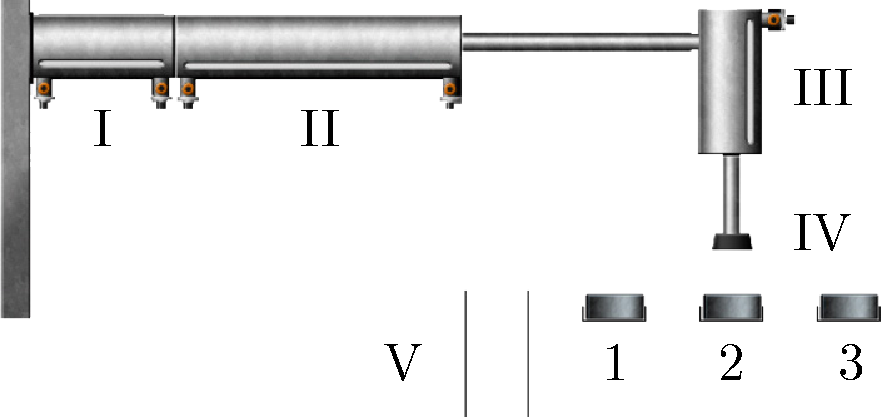
\includegraphics[width=8cm]{pnp-manipulator.pdf}
    \caption{Pick-and-Place манипулятор}%
    \label{fig:pnp-manipulator}
\end{figure}

Pick-and-Place (PnP) манипулятор, изображенный на рисунке~\ref{fig:pnp-manipulator}, состоит из двух горизонтальных пневматических цилиндров~(I,~II), одного вертикального цилиндра~(III) и захватывающего устройства с вакуумной присоской~(IV) для подъема рабочий деталей.
Когда рабочая деталь оказывается во входном лотке (1,~2,~3), горизонтальные цилиндры располагают актюатор над деталью, вертикальный цилиндр опускает захватывающее устройство, который в свою очередь захватывает деталь, после чего вся система аналогичным образом приходит в движение для переноса захваченной детали в выходной лоток~(V).
Данная система управления реализована в соответствии со стандартом IEC~61499 с использованием функциональных блоков в среде моделирования nxtSTUDIO~\cite{nxtstudio}.
Логический контроллер, осуществляющий управление, выполнен в виде базового функционального блока, интерфейс которого включает в себя одно входное событие \texttt{REQ} (\textit{request}), одно выходное событие \texttt{CNF} (\textit{confirmation}), а также десять входных и семь выходных переменных.
Контроллер PnP\-/манипулятора оперирует следующими входными сигналами~$\SetInputVariables$, поступающими от объекта управления \--- среды исполнения:
\begin{itemize}[nosep]
    \item \texttt{c1Home}/\texttt{c1End} \--- горизонтальный цилиндр~I находится в крайнем левом/правом положении;
    \item \texttt{c2Home}/\texttt{c2End} \--- горизонтальный цилиндр~II находится в крайнем левом/правом положении;
    \item \texttt{vcHome}/\texttt{vcEnd} \--- вертикальный цилиндр~III находится в крайнем верхнем/нижнем положении;
    \item \texttt{pp1}/\texttt{pp2}/\texttt{pp3} \--- рабочая деталь находится на входном лотке~1/2/3;
    \item \texttt{vac} \--- вакуумная присоска включена.
\end{itemize}
В свою очередь контроллер PnP\-/манипулятора может посылать следующие сигналы~$\SetOutputVariables$ объекту управления:
\begin{itemize}[nosep]
    \item \texttt{c1Extend}/\texttt{c1Retract} \--- удлинить/\allowbreak{}втянуть цилиндр I;
    \item \texttt{c2Extend}/\texttt{c2Retract} \--- удлинить/\allowbreak{}втянуть цилиндр II;
    \item \texttt{vcExtend} \--- удлинить цилиндр III;
    \item \texttt{vacuum\_on}/\texttt{vacuum\_off} \--- включить/выключить ваккумную присоску.
\end{itemize}

% Данное исследование было нацелено на исследование практической применимости разработанных методов на примере синтеза описанного логического контроллера PnP\-/манипулятора.
% Процесс сбора сценариев исполнения (трассировок) для системы PnP\-/манипулятора описан в~\cite{fbCSP}.
% В данной работе были использованы наборы сценариев выполнения различных размеров: 1,~4, 10, 39 и 49 сценариев в каждом.


\subsection{Синтез минимальной конечно-автоматной модели по примерам поведения}%
\label{sub:exp-mono-pnp-scenarios-only}

Для исследования эффективности и практической применимости разработанных методов синтеза минимальных моделей по примерам поведения, производится сравнение с двухэтапным подходом из~\cite{chivilikhin-19}, где на первом этапе производится построение базовой модели, удовлетворяющей заданым сценариям выполнения, с помощью SAT-решателя, а затем охранные условия полученной модели минимизируются с помощью CSP-решателя.
Стоит отметить, что превосходство данного двухэтапного метода над другими методами, например, EFSM-tools~\cite{efsm-tools}, уже было показано в~\cite{chivilikhin-19}, поэтому сравнение происходит только с двухэтапным методом, впоследствии называемым \enquote{Two-stage}.

%% Table: Results for Extended-min-UB
\begin{table}
    \centering
    \caption{Результаты синтеза минимальной конечно-автоматной модели логического контроллера PnP\-/манипулятора по примерам поведения с помощью двухэтапного метода Two-stage~\cite{chivilikhin-19} и алгоритма $\AlgoExtendedMinUB$}%
    \label{tab:results-monolith-pnp-extminub}
    \subfile{tex/tab-mono-pnp-extminub-results}
\end{table}

Для синтеза минимальной конечно-автоматной модели контроллера PnP\-/манипулятора по заданным сценариям выполнения $\SetPositiveScenarios$ был применен алгоритм $\AlgoExtendedMinUB(\SetPositiveScenarios, w)$ с различными значениями параметра~$w$ \--- ширины плато для поиска локального минимума: $w = 0$ для случая, когда первое найденное решение считается финальным, $w = \infty$ для нахождения глобально-минимального решения, а также $w = 2$ для случая использования предложенной эвристики.
Результаты эксперимента представлены в таблице~\ref{tab:results-monolith-pnp-extminub}, где
$\SetPositiveScenarios$ \=== набор сценариев выполнения,
$\card{\PositiveTree}$ \=== размер дерева сценариев;
\enquote{Время, с} \--- время работы в секундах,
$\Nmin$ \=== минимальный суммарный размер охранных условий;
для метода Two\=/stage~\cite{chivilikhin-19}:
$\Cmin$ \=== минимальное число состояний,
$\Tmin$ \=== минимальное число переходов;
для метода $\AlgoExtendedMinUB$:
минимальное число состояний опущено, так как совпадает с $\Cmin$ для двухэтапного метода,
$P$ \=== максимальный размер каждого охранного условия,
$T$ \=== число переходов (не было минимизировано),
$w$ \=== критическая ширина плато для предложенной эвристики.
Результаты свидетельствуют о том, что разработанный метод $\AlgoExtendedMinUB$ способен генерировать более компактные конечные автоматны, чем двухэтапный метод, при этом значения эвристического параметра $w = 2$ достаточно для получения оптимального результата в терминах~$\Nmin$.


\subsection{Синтез минимальной конечно-автоматной модели по примерам поведения и LTL-спецификации}%
\label{sub:exp-mono-pnp-with-ltl}

%% Table: LTL properties
\begin{table}[p]
    \centering
    \caption{Темпоральные свойства для системы PnP\-/манипулятора}%
    \label{tab:ltl-properties}
    \begin{adjustbox}{max width=\textwidth, max height=\maxheight{1}}
        \subfile{tex/tab-ltl-properties}
    \end{adjustbox}
\end{table}

Следующий эксперимент посвящен учету формальной спецификации с помощью применения индуктивного синтеза, основанного на контрпримерах.
Для использования LTL-свойств \emph{живости} (\textit{liveness}) верификация моделей с помощью NuSMV проводилась в замкнутом цикле~\cite{closed-loop} с заранее подготовленной формальной моделью объекта управления \--- PnP\-/манипулятора.
Эта модель определяет состояние объекта управления в зависимости от команд управления контроллера \--- синтезированной конечно-автоматной модели.
Набор использованых LTL-свойств представлен в таблице~\ref{tab:ltl-properties} и включает в себя как свойства безопасности \Prop{1}\==\Prop{6} (\enquote{система не окажется в нежелательном состояния}), так и свойства живости \Prop{7}\==\Prop{10} (\enquote{что-то полезное когда-нибудь произойдет}).
При этом свойства $\PropertiesConst$ зафиксированы, то есть используются во всех экспериментах, а использование свойств $\PropertiesVar$ разнится.
Стоит отметить, что эти три свойства определяют тот факт, что если рабочая деталь (1\==3) размещается на входном лотке, то она когда-нибудь будет обработана.
Однако в оригинальной системе PnP\-/манипулятора~\cite{patil-pnp} выполняется \emph{только} свойство~\PropWP{1}, касающееся первой детали \--- если в первом входном лотке всегда присутствует рабочая деталь (при ее подъеме на ее месте в этот же момент появляется новая), то рабочие детали во втором и третьем входных лотках никогда не будут обработаны, что нарушает свойства живости \PropWP{2}~и~\PropWP{3}.
Поэтому каждое дополнительное (по отношению к~$\PropertiesConst$) свойство~$\PropertiesVar$ рассматривается отдельно от остальных, при этом предполагается, что рабочие детали появляются только на соответствующих входных лотках.
Для эксперимента с использованием дополнительного LTL-свойства~\PropWP{2} был использован специальный набор сценариев $\SetScenarios^{(1)\prime\prime}$, состоящий из одного сценария, описывающего обработку детали во втором входном лотке.
Аналогично, для свойства~$\PropWP{3}$ был использован специальный набор сценариев $\SetScenarios^{(1)\prime\prime\prime}$, состоящий из одного сценария, описывающего обработку детали в третьем входном лотке.

Проведенное экспериментальное сравнение включало в себя три метода: два разработанных метода $\AlgoCegis$ и $\AlgoCegisMin$, входящие в состав \smallcaps{fbSAT}, а также расширение метода \smallcaps{fbCSP} для учета LTL\-/спецификации, называемое впоследствии \mbox{\smallcaps{fbCSP+LTL}}~\cite{chivilikhin-18}.
Для обоих разработанных методов параметры $C^{*}$~и~$P^{*}$ были предварительно оценены с помощью алгоритма $\AlgoExtendedMinUB$ с параметром $w = 2$, время работы было учтено в суммарном времени работы алгоритма CEGIS\@.
% Для обоих разработанных методов использовалось значение параметра $w = 2$, эффективность которого была показана ранее (раздел~\ref{sub:exp-mono-pnp-scenarios-only}).
% Помимо времени работы методов и значения суммарного размера охранных условий $N$, также было учтено число итераций CEGIS\@.
Дополнительно, синтезированные модели были вручную протестированы в nxtSTUDIO~\cite{nxtstudio} \--- загружены в симуляционную среду и проверены на соответствие желаемому поведению.
Результаты данного экспериментального исследования представлены в таблице~\ref{tab:results-monolith-pnp-cegis}, где
\enquote{Дополнительное LTL-свойство} \--- одно из свойств $\PropertiesVar$, использованное в дополнение к свойствам $\PropertiesConst$,
$\SetPositiveScenarios$ \=== набор использованых позитивных сценариев выполнения $\SetPositiveScenarios$,
$N_{\text{init}}$ \--- начальный минимальный суммарный размер охранных условий (для автомата, полученного с помощью алгоритма $\AlgoExtendedMinUB(\SetPositiveScenarios, w)$),
\enquote{Время, с} \--- время работы в секундах,
$P$ \=== максимальный размер охранного условия,
$N$ \=== финальный суммарный размер охранных условий (при использовании алгоритма $\AlgoCegisMin$ это значения является минимальным),
\enquote{\#iter} \--- число итераций CEGIS\@.

%% Table: Results for CEGIS
\begin{table}
    \centering
    \caption{Результаты применения подхода CEGIS к синтезу конечно-автоматной модели логического контроллера PnP\-/манипулятора по примерам поведения и LTL\-/спецификации}%
    \label{tab:results-monolith-pnp-cegis}
    \subfile{tex/tab-mono-pnp-cegis-results}
\end{table}

Анализируя полученные результаты, можно заметить, что модели, найденные с помощью подхода CEGIS всегда имеют больший размер (в терминах суммарного размера охранных условий~$N$), нежели модели, построенные только по сценариям выполнения.
Это объясняется тем, что используемые сценарии выполнения не полностью покрывают рассмотренную LTL\-/спецификацию.
Поэтому алгоритм $\AlgoCegisMin$ всегда находит наименьшее решение и во всех случаях превосходит \mbox{\smallcaps{fbCSP+LTL}}~\cite{chivilikhin-18}, как по времени работы, так и по размеру моделей.
Наиболее интересным результатом является то, что $\AlgoCegisMin$ позволяет эффективно синтезировать модели по наборам сценариев $\SetScenarios^{(1)}$, $\SetScenarios^{(1)\prime\prime}$ и $\SetScenarios^{(1)\prime\prime\prime}$ \--- эти сценарии \enquote{не~покрывают} соответствующие свойства живости $\PropertiesVar$ в том смысле, что эти сценарии описывают процесс обработки только одной рабочей детали.
Существующий метод \smallcaps{fbCSP+LTL}~\cite{chivilikhin-18} не~справился в этих случаях, в то время как разработанный метод $\AlgoCegisMin$ с легкостью преуспел.
Также стоит отметить, что алгоритм $\AlgoCegis$ позволяет синтезировать модели быстрее, однако не обеспечивает минимальности охранных условий.


\section{Экспериментальное исследование: SYNTCOMP}%
\label{sec:experiments-monolith-syntcomp}

%% Weird boolvec notation from the original BoSy paper
\newcommand{\myboolvec}[1]{2^{#1}}

В этом разделе описывается применение разработанных методов к задаче синтеза системы переходов (\textit{transition system})~\cite{bosy,not-bosy} по входным данным с соревнования по реактивному синтезу SYNTCOMP~\cite{syntcomp}.
Один из треков соревнования SYNTCOMP \--- трек последовательного синтеза (\textit{sequential synthesis track}) \--- посвящен задаче синтеза системы переходов по заданной LTL\-/спецификации, также известной как задача LTL-синтеза.
Существует множество различных программных средств, осуществляющих LTL-синтез, среди которых можно выделить BoSy~\cite{bosy,not-bosy} и Strix~\cite{strix}.
Стоит отметить, что среди всех доступных программных средств только BoSy ограничивает размеры (число состояний) генерируемых систем переходов, однако BoSy не минимизирует размеры охранных условий, что значительно затрудняет анализ получаемых систем человеком.
Также стоит отметить, что на текущий момент разработанное в данной работе программное средство \smallcaps{fbSAT} неприменимо в явном виде к задаче LTL-синтеза, так как для \smallcaps{fbSAT} необходимым условием является наличие некоторого множества позитивных сценариев выполнения~$\SetPositiveScenarios$.
Несмотря на это, \smallcaps{fbSAT} может быть применен для \emph{минимизации} систем переходов, генерируемых BoSy.

Формально\footnote{%
    Здесь стоит отметить, что в данном разделе для описания системы переходов используется \emph{оригинальная} нотация из~\cite{not-bosy}.
    Эта нотация может конфликтовать с другими частями данной работы \--- следует считать, что все объявления в данном разделе действуют только здесь.
    Также стоит отметить, что в оригинальной нотации для обозначения \textit{множества всех наборов значений} пропозициональных переменных используется нотация $\myboolvec{X}$, где $X$ \--- множество пропозициональных переменных, однако более корректным обозначением было бы $\boolvec{X}$.
},
\textit{система переходов}~$\mathcal{T}$ это кортеж $\Tuple{ T, t_0, \Sigma = I \union O, \tau }$, где
$T$ \=== множество состояний,
$t_0 \in T$ \=== стартовое состояние,
$\Sigma$ \=== алфавит системы,
$I$ \=== множество пропозициональных переменных, управляемых окружением (\textit{входы}),
$O$ \=== множество пропозициональных переменных, управляемых системой (\textit{выходы}),
$\tau \colon T \times \myboolvec{I} \to \myboolvec{O} \times T$ \--- функция перехода, отображающая состояние~$t$ и входной набор $\bm{i} \in \myboolvec{I}$ в выходной набор $\bm{o} \in \myboolvec{O}$ и новое состояние~$t'$.
% $\Pair{t, \bm{i}} \mapsto \Pair{\bm{o}, t'}$
Можно заметить сходство систем переходов и конечно-автоматных моделей ECC базовых функциональных блоков.
Если система переходов обладает семантикой, схожей с семантикой автомата Мура (то есть выходы в функции перехода зависят от состояния системы), то такая система может быть смоделирована в виде ECC, а значит и синтезирована с помощью \smallcaps{fbSAT}\@.

% \begin{equation}
%     \label{eq:moore-condition}
%     \forall t \in T
%     \ldotp
%     \forall \bm{i} \neq \bm{i}' \in \myboolvec{I}
%     \ldotp
%     \bigl[
%         \tau(t, \bm{i}) = \Pair{\bm{o}, \_\,}
%         \land
%         \tau(t, \bm{i}') = \Pair{\bm{o}', \_\,}
%     \bigr]
%     \implies
%     (\bm{o} = \bm{o}')
% \end{equation}

Наборы данных (\textit{инстансы}) на соревновании SYNTCOMP представляют собой JSON-файлы с описанием интерфейса системы и набора инвариантов \--- свойств на языке LTL, которые должны выполняться в каждый момент времени работы системы.
В листинге~\ref{lst:lilydemo19-json} приведен пример инстанса \texttt{lilydemo19}, описывающего систему с семантикой автомата Мили. Данная система оперирует входами $\Set{\texttt{ec}, \texttt{ets}}$ и выходами $\Set{\texttt{fl}, \texttt{hl}}$.
% В листинге~\ref{lst:full-arbiter-3-json} приведен пример инстанса \texttt{full\_arbiter\_3}, описывающего систему с семантикой автомата Мили. Данная система оперирует входами $\Set{r_0, r_1, r_2}$ и выходами $\Set{g_0, g_1, g_2}$.
Логика работы системы описывается с помощью LTL-свойств, указанных в поле \texttt{guarantees}, а дополнительные глобальные ограничения (предположения) записаны в поле \texttt{assumptions}.

% TODO: fix listing
% \lstinputlisting[
%     float=!htb,
%     language=json,
%     % basicstyle=\small\ttfamily,
%     caption={Инстанс \texttt{lilydemo19.json}},
%     label={lst:lilydemo19-json}
% ]{data/lilydemo19.json}

%%% \lstinputlisting[
%%%     float=!htb,
%%%     language=json,
%%%     % basicstyle=\small\ttfamily,
%%%     caption={Инстанс \texttt{full\_arbiter\_3.json}},
%%%     label={lst:full-arbiter-3-json}
%%% ]{data/full_arbiter_3.json}

При выполнении данной работы был использован набор из 136 инстансов с соревнования SYNTCOMP~2018.
Для получения конечно-автоматных моделей в формате NuSMV по имеющимся LTL\-/спецификациям было использовано программное средство BoSy (input-symbolic, QBF-encoding, максимальное число состояний:~10, максимальное время работы:~1~час), в результате чего только только для 97 из~136 инстансов были получены результирующие модели.
В листинге~\ref{lst:lilydemo19-smv} приведена NuSMV модель для инстанса \texttt{lilydemo19}.
Все полученные модели были просимулированы с помощью NuSMV с целью получения случайных сценариев выполнения различных длин.
Для этого была использована команда `\verb/simulate -r -k <length>/' для симуляции (где `\verb/<length>/' \--- число шагов симуляции) и команда `\verb/show_traces -a -v/' для сохранения трассировок.
% TODO: restore this sentence after re-introducing the section {sec:scenarios}
% Полученные трассировки были сконвертированы в сценарии выполнения в соответствии с разделом~\ref{sec:scenarios}.

% TODO: fix listing
% \lstinputlisting[
%     float=!htb,
%     language=nusmv,
%     % basicstyle=\small\ttfamily,
%     caption={NuSMV модель для инстанса \texttt{lilydemo19}, сгенерированная BoSy},
%     label={lst:lilydemo19-smv}
% ]{data/lilydemo19.smv}

%%% \lstinputlisting[
%%%     float=!htb,
%%%     language=nusmv,
%%%     caption={NuSMV модель для инстанса \texttt{full\_arbiter\_3}, полученная с помощью BoSy},
%%%     label={lst:full-arbiter-3-smv}
%%% ]{data/full_arbiter_3.smv}

Полученные сценарии выполнения были использованы для синтеза конечно-автоматных моделей с помощью \smallcaps{fbSAT}.
На рисунке~\ref{fig:lilydemo19} представлена синтезированная модель для описанного выше инстанса \texttt{lilydemo19}.
Для синтеза было использовано пять сценариев длины~10 (\texttt{scenarios-k5-l10}), алгоритм $\AlgoExtendedMinUB(w = 0)$, время синтеза составило менее секунды.
Модель состоит из $C = 2$ состояний и $T = 4$ переходов, а охранные условия имеют суммарный размер $N = 6$.
Дополнительный этап верификации подтвердил соответствие синтезированной системы исходной LTL\-/спецификации, указанной во входном файле \texttt{lilydemo19.json}.
Как можно заметить, синтезированная модель полностью эквивалентна исходной NuSMV модели, поэтому необходимо рассмотрение более \enquote{сложного} инстанса.

%% Picture: lilydemo19 synthesized model
\begin{figure}[htb]
    \centering
    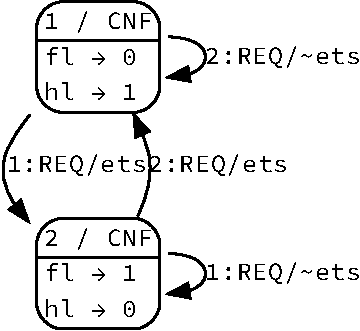
\includegraphics[max width=\textwidth]{lilydemo19.pdf}
    \caption{Конечно-автоматная модель для инстанса \texttt{lilydemo19}, синтезированная с помощью \smallcaps{fbSAT}}%
    \label{fig:lilydemo19}
\end{figure}

Рассмотрим инстанс \texttt{full\_arbiter\_3} \--- данная система оперирует входами $\Set{r_0, r_1, r_2}$ и выходами $\Set{g_0, g_1, g_2}$.
Полученная с помощью BoSy система переходов $\mathcal{T}_{\text{original}}$ изображена на рисунке~\ref{fig:syntcomp-bosy} и состоит из $C = 8$ состояний и $T = 28$ переходов, а суммарный размер охранных условий $N = 147$.
На этом этапе можно предположить, что полученная модель не является минимальной, а значит, возможно применение \smallcaps{fbSAT} для синтеза минимальной модели, также соответствующей исходной LTL\-/спецификации \--- для этого был использован алгоритм $\AlgoCegisMin$.
Стоит заметить, что для более эффективного синтеза необходимо полное покрытие состояний сценариями выполнения. Поэтому было использовано 20~сценариев, каждый длины~20 (\texttt{scenarios-k20-l20}).

Стоит отметить, что формальное определение системы переходов, данное выше, не обязывает функцию переходов $\tau$ быть детерминированной, однако \smallcaps{fbSAT} всегда генерирует детерминированные модели.
Также стоит отметить, что формальное определение системы переходов не включает в себя функцию приоритета переходов, которая присутствует в определении ECC\@.
Для того, чтобы модели, синтезируемые \smallcaps{fbSAT}, соответствовали моделям, получаемым с помощью BoSy, в \smallcaps{fbSAT} было добавлено ограничение на \enquote{дизъюнктивные переходы}\footnote{Флаг \texttt{-{}-encode-disjunctive-transitions} в \smallcaps{fbSAT}} \--- в каждом состоянии $q \in \SetStates$ для каждого входа $u \in \SetTreeInputs$ выполняется не более одного перехода.
В результате была синтезирована модель $\Automaton_{\text{deterministic}}$, изображенная на рисунке~\ref{fig:syntcomp-fbsat-deterministic}, с тем же числом состояний и переходов, что и $\mathcal{T}_{\text{original}}$, однако с меньшим суммарным размером охранных условий: $N = 105$.

Если же не использовать введенное ограничение на \enquote{дизъюнктивные переходы}, то есть использовать \smallcaps{fbSAT} в оригинальном виде, то синтезируемые модели будут детерминированными ECC (из-за функции приоритета переходов), но недетерминированными системами переходов.
В таком случае результирующая модель $\Automaton_{\text{non-deterministic}}$, изображенная на рисунке~\ref{fig:syntcomp-fbsat}, обладает наименьшим суммарным размером охранных условий: $N = 52$.

Полученные результаты показывают, что предложенный подход к явному кодированию деревьев разбора булевых формул, соответствующих охранным условиям на переходах автомата, позволяет существенно сократить суммарный размер охранных условий в автомате.
Стоит также отметить, что данный подход применим не только \emph{после} LTL-синтеза \--- возможно расширить SAT-/QBF-сведение в BoSy предложенной кодировкой для охранных условий для их минимизации непосредственно \emph{в процессе} синтеза.


\chapterconclusion

В данной главе была рассмотрена задача синтеза монолитных конечно-автоматных моделей логических контроллеров по примерам поведения и формальной спецификации.
Для решения этой задачи были разработаны методы, основанные на сведении к задаче выполнимости SAT и применении SAT-решателей.
Отдельное внимание было уделено решению задачи синтеза минимальных моделей.
Разработанные методы были реализованы в виде программного средства \smallcaps{fbSAT}~\cite{fbSAT-tool}.
Работоспособность и эффективность разработанных методов были проверены в ходе экспериментального исследования, посвященному синтезу модели логического контроллера, управляющего Pick-and-Place манипулятором.
Дополнительно, разработанные методы были применены для минимизации конечно-автоматных моделей, получаемых в ходе LTL-синтеза с помощью программного средства BoSy по исходным данным с соревнования по реактивному синтезу SYNTCOMP\@.



\FloatBarrier
